\documentclass[acmsmall,screen,nonacm]{acmart}
\usepackage[greek,english]{babel}
\usepackage{float}

\babelfont[greek]{rm}{Noto Serif}
\babelfont[greek]{sf}{Noto Sans}
\sloppy
\title{Εφαρμογή online παραγγελίας φαγητού(LogoFood)}


\author{Εμμανουήλ Παξιμαδάκης 1100972 \& Δημήτριος Φιλόπουλος 1101130}
\affiliation{
	\institution{\newline Τμήμα ΗΜ\&ΤΥ, Πανεπιστήμιο Πατρών}
	\country{Ελλάδα}
}
\captionsetup[table]{position=bottom}

\renewcommand{\shortauthors}{Ε.Π., Δ.Φ.}

\begin{document}
	
	% --- ΠΕΡΙΛΗΨΗ ---
	\begin{abstract}
		\textbf{Περίληψη:} Η παρούσα εργασία παρουσιάζει την ανάπτυξη της web εφαρμογής LogoFeet στα πλαίσια του μαθήματος "Προγραμματισμός Διαδικτύου". Η εφαρμογή εξελίχθηκε από ένα αρχικό λειτουργικό πρωτότυπο (static HTML/CSS) σε μια πλήρη Full-Stack εφαρμογή που χρησιμοποιεί Node.js, Express και Handlebars, υποστηρίζοντας δυναμική διαχείριση δεδομένων και γεωχωρικές λειτουργίες.
	\end{abstract}
	
	\maketitle
	
	\section{Εισαγωγή}
	Σκοπός του project είναι η εξοικείωση με τις σύγχρονες τεχνολογίες διαδικτύου για τη δημιουργία μιας δυναμικής πλατφόρμας παραγγελιοληψίας. Η ανάπτυξη ακολούθησε μια σταδιακή προσέγγιση, ξεκινώντας από το σχεδιασμό της διεπαφής και καταλήγοντας στην υλοποίηση σύνθετης επιχειρησιακής λογικής στο backend.
	
	\section{Λειτουργικές Απαιτήσεις και Σενάρια Χρήσης}
	Το σύστημα σχεδιάστηκε για να καλύπτει πλήρως τον κύκλο ζωής μιας παραγγελίας, εξυπηρετώντας δύο διακριτούς ρόλους (Πελάτης και Εστιατόριο). Οι κύριες λειτουργικές απαιτήσεις περιλαμβάνουν:

	\subsection{Λειτουργίες Πελάτη}
	\begin{itemize}
		\item \textbf{Αναζήτηση \& Φιλτράρισμα:} Δυνατότητα εύρεσης εστιατορίων που εξυπηρετούν τη συγκεκριμένη τοποθεσία (ακτίνα 4χλμ) μέσω ενσωμάτωσης χάρτη και φιλτραρίσματος βάσει κατηγοριών κουζίνας.
		\item \textbf{Διαχείριση Προφίλ \& Διευθύνσεων:} Εγγραφή, σύνδεση, και δυνατότητα αποθήκευσης πολλαπλών διευθύνσεων παράδοσης.
		\item \textbf{Διαχείριση Καλαθιού \& Checkout:} Προσθήκη προϊόντων, υπολογισμός συνόλου με μεταφορικά και ολοκλήρωση παραγγελίας, η οποία είναι διαθέσιμη ακόμα και για επισκέπτες (Guest Checkout).
		\item \textbf{Live Tracking \& Αξιολόγηση:} Παρακολούθηση της πορείας της παραγγελίας σε πραγματικό χρόνο και δυνατότητα αξιολόγησης του εστιατορίου μετά την ολοκλήρωση.
	\end{itemize}

	\subsection{Λειτουργίες Εστιατορίου}
	\begin{itemize}
		\item \textbf{Διαχείριση Καταλόγου (Menu):} Προσθήκη, επεξεργασία, διαγραφή προϊόντων, εικόνων, τιμών και ένταξή τους σε κατηγορίες.
		\item \textbf{Dashboard Παραγγελιών:} Πίνακας ελέγχου για την παραλαβή νέων παραγγελιών και την ενημέρωση της κατάστασής τους (π.χ., PREPARING, DELIVERING).
		\item \textbf{Ρυθμίσεις Καταστήματος:} Καθορισμός ελάχιστης παραγγελίας και διαχείριση της συνολικής κατάστασης λειτουργίας.
	\end{itemize}

	\section{Αρχιτεκτονική Model-View-Controller (MVC)}
	Για τη βέλτιστη οργάνωση, συντηρησιμότητα και επεκτασιμότητα του κώδικα, η αρχιτεκτονική της εφαρμογής δομήθηκε αυστηρά πάνω στο σχεδιαστικό πρότυπο \textbf{Model-View-Controller (MVC)}. Αυτός ο διαχωρισμός αρμοδιοτήτων επιτρέπει την ανεξάρτητη ανάπτυξη της διεπαφής χρήστη, της επιχειρησιακής λογικής και της διαχείρισης δεδομένων.
	
	\subsection{Επίπεδο Δεδομένων (Model)}
	Το επίπεδο \textbf{Model} (\texttt{/model}) είναι αποκλειστικά υπεύθυνο για την αλληλεπίδραση με τη βάση δεδομένων και την υλοποίηση των κανόνων της επιχειρησιακής λογικής (business logic).
	Στην υλοποίησή μας, δημιουργήθηκαν εξειδικευμένα αρχεία (π.χ., \texttt{auth-model.mjs}, \texttt{order-model.mjs}, \texttt{restaurant-model.mjs}) τα οποία εκτελούν παραμετροποιημένα ερωτήματα SQL (Parameterized Queries) μέσω του MySQL driver. Αυτή η αφαίρεση (abstraction) εξασφαλίζει ότι το υπόλοιπο σύστημα αγνοεί τις ιδιαιτερότητες της βάσης δεδομένων, ενώ ταυτόχρονα παρέχει προστασία από επιθέσεις SQL Injection.
	
	\subsection{Επίπεδο Παρουσίασης (View)}
	Το επίπεδο \textbf{View} (\texttt{/views}) αναλαμβάνει την οπτική αναπαράσταση των δεδομένων στον τελικό χρήστη.
	Αντί για στατικά HTML αρχεία, χρησιμοποιήθηκε η μηχανή δημιουργίας προτύπων (template engine) \textbf{Handlebars} (\texttt{.hbs}). Η προσέγγιση αυτή προσφέρει πολλαπλά πλεονεκτήματα:
	\begin{itemize}
		\item \textbf{Δυναμική Δημιουργία Περιεχομένου:} Επιτρέπει την ενσωμάτωση μεταβλητών, βρόχων (\texttt{\{\{\#each\}\}}) και δομών ελέγχου (\texttt{\{\{\#if\}\}}) απευθείας στο HTML markup.
		\item \textbf{Επαναχρησιμοποίηση Κώδικα:} Η χρήση ενός κεντρικού \texttt{layout} (\texttt{main.hbs}) και επιμέρους τμημάτων (partials) μειώνει τον πλεονάζοντα κώδικα και διευκολύνει τις καθολικές αλλαγές στο UI (π.χ. στο header ή το footer).
	\end{itemize}

	\subsection{Επίπεδο Ελέγχου (Controller)}
	Το επίπεδο \textbf{Controller} (\texttt{/controller}) λειτουργεί ως ο ενδιάμεσος "τροχονόμος" (router) μεταξύ του χρήστη, του Model και του View. 
	Κάθε ξεχωριστή οντότητα του συστήματος διαθέτει τον δικό της ελεγκτή (π.χ., \texttt{cart-controller.mjs}, \texttt{index-controller.mjs}). Οι Controllers είναι υπεύθυνοι για:
	\begin{enumerate}
		\item Την παραλαβή και επικύρωση (validation) των HTTP αιτημάτων (GET, POST, κ.λπ.) από τον Client.
		\item Την κλήση των κατάλληλων μεθόδων του Model για ανάκτηση ή αποθήκευση δεδομένων.
		\item Την προετοιμασία των δεδομένων (data formatting) και την προώθησή τους στο κατάλληλο View για τελική απόδοση (render) ή την εκτέλεση ανακατευθύνσεων (redirects).
	\end{enumerate}

	\section{Σχεδιασμός Βάσης Δεδομένων}
	Η βάση δεδομένων της εφαρμογής είναι σχεσιακή (RDBMS) και αποτελείται από πίνακες που απεικονίζουν τις βασικές οντότητες του συστήματος και τις μεταξύ τους σχέσεις. Τα βασικά δομικά στοιχεία είναι:
	\begin{itemize}
		\item \textbf{Users \& Roles:} Διαχείριση λογαριασμών (Πελάτες, Εστιατόρια) με χρήση διακριτών ρόλων.
		\item \textbf{Address:} Αποθήκευση συντεταγμένων (Latitude/Longitude) και πλήρους κειμένου διεύθυνσης για την υποστήριξη των γεωχωρικών αναζητήσεων.
		\item \textbf{Menu \& Categories:} Οργάνωση των διαθέσιμων προϊόντων κάθε εστιατορίου ανά κατηγορία.
		\item \textbf{Orders \& Order\_Items:} Καταγραφή του ιστορικού παραγγελιών, με λεπτομέρειες για το κάθε προϊόν, τη διεύθυνση παράδοσης (μέσω snapshot) και το status της παραγγελίας.
		\item \textbf{Reviews:} Αποθήκευση βαθμολογιών για τον υπολογισμό του μέσου όρου (rating) κάθε εστιατορίου.
	\end{itemize}
	
	\begin{figure}[h]
		\centering
		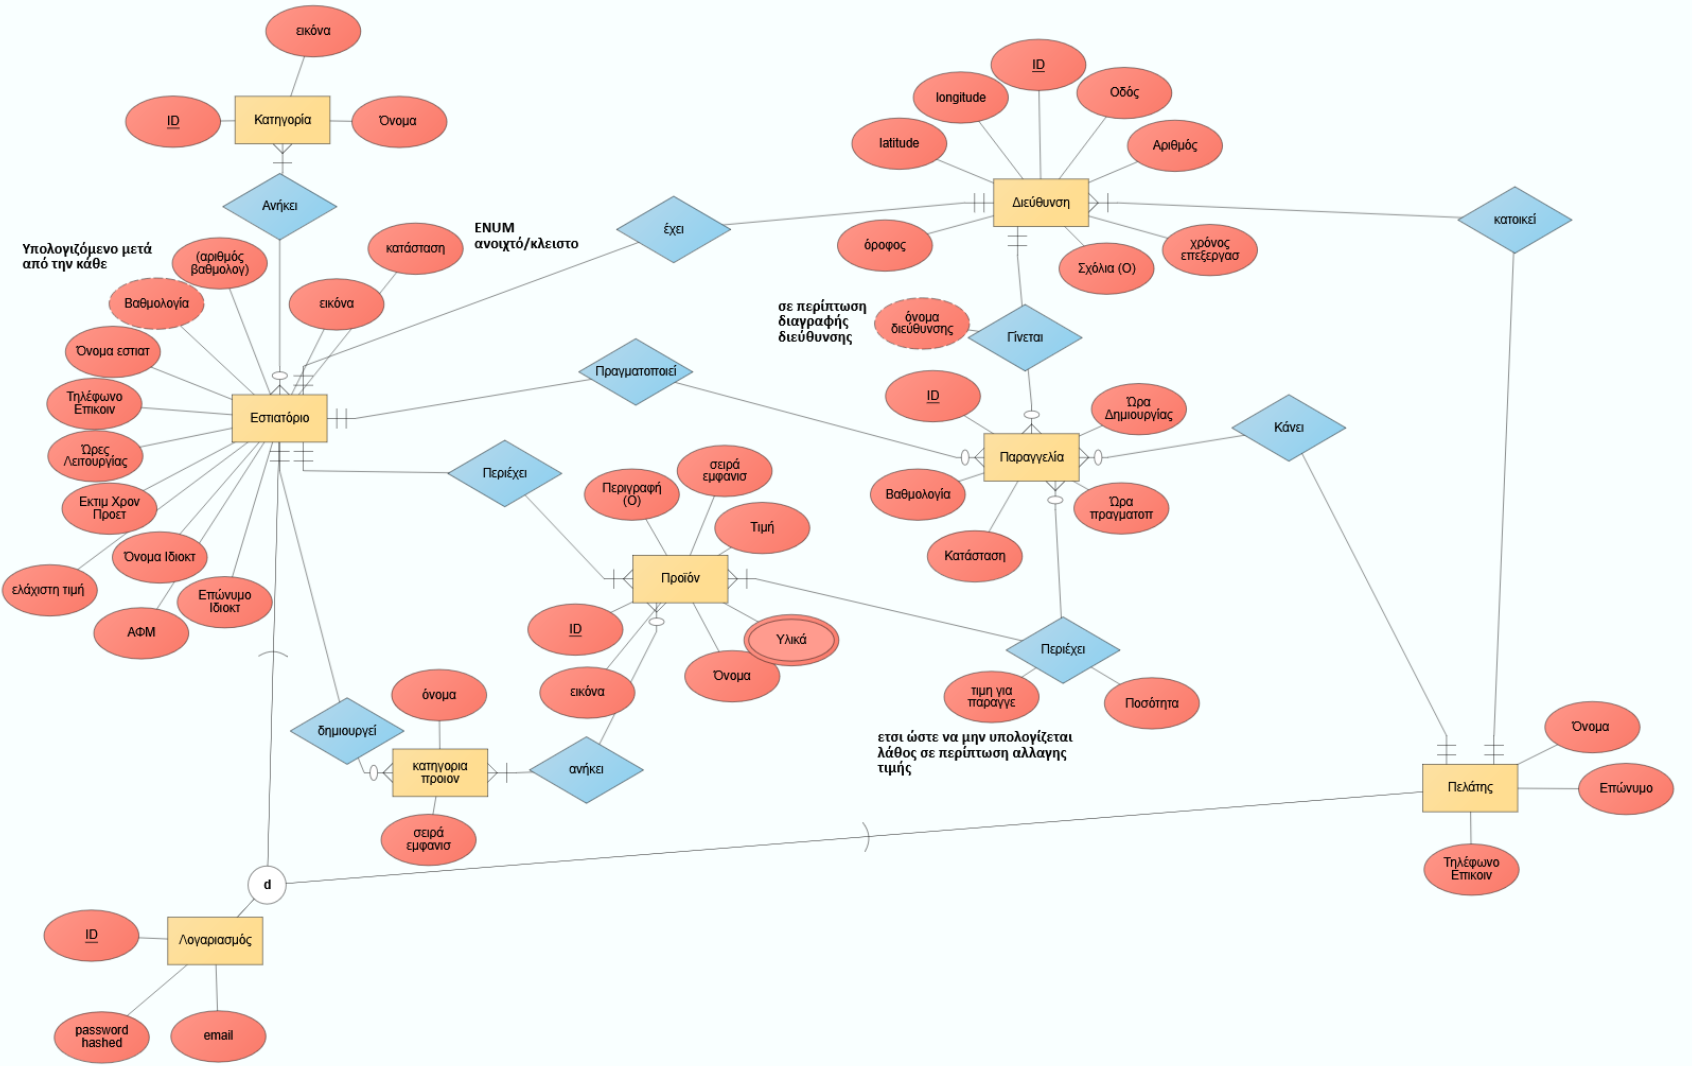
\includegraphics[width=0.9\linewidth]{images/er_diagram.png}
		\caption{Το διάγραμμα σχέσεων-οντοτήτων της βάσης δεδομένων.}
	\end{figure}
	
	\begin{figure}[h]
		\centering
		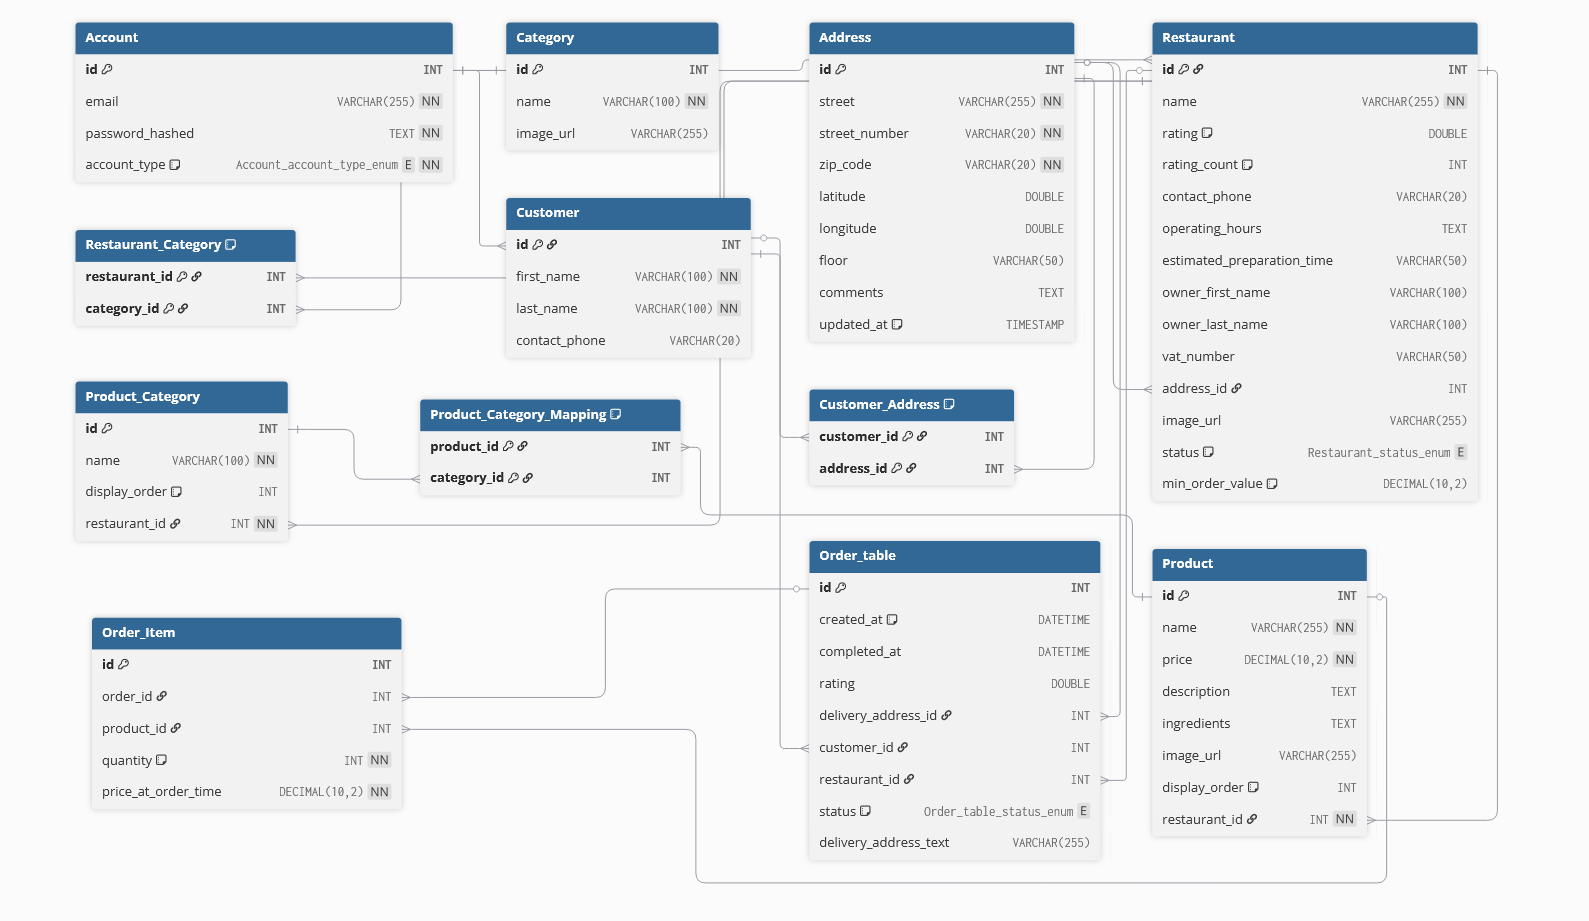
\includegraphics[width=0.9\linewidth]{images/schema.png}
		\caption{Schema της βάσης δεδομένων.}
	\end{figure}

	\section{Τεχνολογίες Υλοποίησης}
	
	\subsection{Frontend (Διεπαφή Χρήστη)}
	Για τη διεπαφή επιλέχθηκαν τεχνολογίες που εξασφαλίζουν ταχύτητα και συμβατότητα:
	\begin{itemize}
		\item \textbf{Bootstrap 5 \& Vanilla CSS:} Χρησιμοποιήθηκαν για τη δημιουργία ενός μοντέρνου, responsive σχεδιασμού (mobile-first approach). Η χρήση έτοιμων components της Bootstrap (cards, modals, alerts) επιτάχυνε σημαντικά την ανάπτυξη.
		\item \textbf{Handlebars (HBS):} Ως μηχανή προτύπων επέτρεψε την καθαρή ενσωμάτωση δυναμικών δεδομένων στα HTML αρχεία.
		\item \textbf{Leaflet.js \& OpenStreetMap:} Αποτέλεσαν τη βάση για τη διαδραστική απεικόνιση χαρτών και την επιλογή τοποθεσιών, αποτελώντας μια ισχυρή, open-source εναλλακτική έναντι των κλειστών εμπορικών λύσεων.
	\end{itemize}
	
	\subsection{Backend (Εξυπηρετητής)}
	Η "καρδιά" του συστήματος αναπτύχθηκε σε περιβάλλον JavaScript, επιτρέποντας πλήρη ομοιογένεια (Isomorphic JavaScript) μεταξύ Frontend και Backend:
	\begin{itemize}
		\item \textbf{Node.js \& Express.js:} Το Node.js, χάρη στη μη-μπλοκαρισμένη I/O αρχιτεκτονική του (non-blocking), είναι ιδανικό για την ταυτόχρονη διαχείριση πολλαπλών requests. Το Express.js προσέφερε το απαραίτητο routing και middleware architecture.
		\item \textbf{Middlewares:} Υλοποιήθηκαν custom λύσεις (π.χ., έλεγχος πρόσβασης/authorization) και αξιοποιήθηκαν βιβλιοθήκες όπως το \texttt{express-session} για τη διαχείριση συνεδριών χρήστη.
	\end{itemize}
	
	\subsection{Διαχείριση Δεδομένων και Μετάβαση}
	Στο πρώτο στάδιο ανάπτυξης χρησιμοποιήθηκε η SQLite3 για την ταχεία δημιουργία πρωτοτύπου. Στην τελική έκδοση, η εφαρμογή μεταφέρθηκε σε cloud περιβάλλον (TiDB Cloud) με χρήση MySQL, διασφαλίζοντας κλιμακωσιμότητα και απομακρυσμένη πρόσβαση.
	
	\section{Geospatial Λειτουργίες και Περιορισμοί Απόστασης}
	Ένα από τα κρισιμότερα χαρακτηριστικά της εφαρμογής είναι ο περιορισμός της εμβέλειας παράδοσης των εστιατορίων στα 4 χιλιόμετρα. Για την υλοποίηση αυτής της απαίτησης, αναπτύχθηκε ένα σύστημα που συνδυάζει client-side γεωκωδικοποίηση και server-side επαλήθευση.

	\subsection{Υπολογισμός Απόστασης με τον Τύπο Haversine}
	Για τον ακριβή υπολογισμό της απόστασης μεταξύ του πελάτη και του εστιατορίου στην επιφάνεια της γης, χρησιμοποιήθηκε ο μαθηματικός τύπος \textbf{Haversine}. Ο τύπος αυτός λαμβάνει υπόψη την καμπυλότητα της γης και υπολογίζεται ως εξής:
	\begin{equation}
		a = \sin^2\left(\frac{\Delta\phi}{2}\right) + \cos(\phi_1) \cdot \cos(\phi_2) \cdot \sin^2\left(\frac{\Delta\lambda}{2}\right)
	\end{equation}
	\begin{equation}
		c = 2 \cdot \arctan2(\sqrt{a}, \sqrt{1-a})
	\end{equation}
	\begin{equation}
		d = R \cdot c
	\end{equation}
	όπου $\phi$ είναι το γεωγραφικό πλάτος (latitude), $\lambda$ το γεωγραφικό μήκος (longitude) σε ακτίνια (radians), και $R = 6371 \text{ km}$ η μέση ακτίνα της Γης.

	Η συνάρτηση \texttt{getDistanceKm} υλοποιήθηκε στο αρχείο \texttt{geo-utils.mjs} και καλείται κατά τη διαδικασία του checkout για να διασφαλίσει ότι η παραγγελία δεν υπερβαίνει το όριο των 4 χιλιομέτρων.

	\subsection{Αυτόματo Geocoding}
	Για τη διευκόλυνση του χρήστη, ενσωματώθηκε το API της υπηρεσίας OpenStreetMap (Nominatim). Όταν ο χρήστης πληκτρολογεί τη διεύθυνσή του, το σύστημα εκτελεί ασύγχρονα requests (AJAX) για την εύρεση των συντεταγμένων.

	Κατά την υλοποίηση παρατηρήθηκε ότι αν ο χρήστης άλλαζε τη διεύθυνση χειροκίνητα στα πεδία κειμένου μετά από μια επιλογή στο χάρτη, οι κρυφές συντεταγμένες παρέμεναν οι παλιές. Για την επίλυση αυτού του προβλήματος, προστέθηκαν event listeners που μηδενίζουν τις συντεταγμένες μόλις ο χρήστης τροποποιήσει τα πεδία της διεύθυνσης, αναγκάζοντας το σύστημα να εκτελέσει νέα γεωκωδικοποίηση κατά την υποβολή της φόρμας.

	\section{Παρακολούθηση Παραγγελιών σε Πραγματικό Χρόνο (Live Tracking)}
	Για την αναβάθμιση της εμπειρίας του χρήστη, υλοποιήθηκε ένα σύστημα παρακολούθησης της εξέλιξης της παραγγελίας (Live Tracking). Ο πελάτης μπορεί να βλέπει σε ποιο στάδιο βρίσκεται η παραγγελία του σε πραγματικό χρόνο.

	\subsection{Μηχανή Καταστάσεων Παραγγελίας}
	Η παραγγελία διέρχεται από τις εξής διακριτές καταστάσεις (States), οι οποίες ενημερώνονται από το εστιατόριο μέσω του δικού του Dashboard:
	\begin{itemize}
		\item \textbf{PENDING (10\%):} Η παραγγελία έχει υποβληθεί και εκκρεμεί η αποδοχή της.
		\item \textbf{PREPARING (35\%):} Το εστιατόριο προετοιμάζει τα προϊόντα.
		\item \textbf{READY (60\%):} Τα προϊόντα είναι έτοιμα προς παράδοση.
		\item \textbf{DELIVERING (85\%):} Η παραγγελία βρίσκεται καθ' οδόν προς τον πελάτη.
		\item \textbf{COMPLETED (100\%):} Η παραγγελία παραδόθηκε επιτυχώς.
	\end{itemize}

	Στο frontend (\texttt{track-orders.hbs}), χρησιμοποιήθηκε μια μπάρα προόδου (Progress Bar) της Bootstrap, το πλάτος της οποίας διαμορφώνεται δυναμικά βάσει της κατάστασης της παραγγελίας, προσφέροντας μια συνεχή και κατανοητή οπτική ένδειξη στον χρήστη.

	\subsection{Αρχιτεκτονική Πραγματικού Χρόνου με Server-Sent Events (SSE)}
	Για την υλοποίηση της ενημέρωσης σε πραγματικό χρόνο χωρίς την ανάγκη συνεχούς επαναφόρτωσης της σελίδας από τον χρήστη, επιλέχθηκε η τεχνολογία \textbf{Server-Sent Events (SSE)}. Η επιλογή αυτή κρίθηκε ως η βέλτιστη για τις ανάγκες της εφαρμογής σε σχέση με εναλλακτικές προσεγγίσεις.

	\subsubsection{Σύγκριση και Επιλογή Τεχνολογίας}
	Κατά τη φάση σχεδιασμού εξετάστηκαν τρεις βασικές προσεγγίσεις για την ενημέρωση της κατάστασης των παραγγελιών:
	\begin{itemize}
		\item \textbf{Short Polling (AJAX):} Ο πελάτης στέλνει περιοδικά αιτήματα στον διακομιστή (π.χ. ανά 5 δευτερόλεπτα). Η μέθοδος αυτή απορρίφθηκε ως κύρια λύση λόγω του μεγάλου αριθμού άσκοπων αιτημάτων HTTP που επιβαρύνουν τον διακομιστή και τη βάση δεδομένων όταν δεν υπάρχει αλλαγή κατάστασης.
		\item \textbf{WebSockets:} Επιτρέπουν αμφίδρομη, full-duplex επικοινωνία. Αν και εξαιρετικά ισχυρή τεχνολογία, κρίθηκε υπερβολικά πολύπλοκη για τις συγκεκριμένες ανάγκες, καθώς η επικοινωνία παρακολούθησης είναι αυστηρά μονοκατευθυντική (από τον διακομιστή προς τον πελάτη).
		\item \textbf{Server-Sent Events (SSE):} Πρόκειται για ένα εγγενές πρότυπο του HTML5 που επιτρέπει στον διακομιστή να σπρώχνει (push) δεδομένα προς τον πελάτη μέσω μιας απλής, διαρκούς σύνδεσης HTTP. Προσφέρει χαμηλό overhead, αυτόματη επανασύνδεση (auto-reconnection) από το πρόγραμμα περιήγησης και είναι ιδανικό για μονοκατευθυντική ροή δεδομένων πραγματικού χρόνου.
	\end{itemize}

	\subsubsection{Υλοποίηση στην Πλευρά του Διακομιστή (Server-Side)}
	Στο backend της εφαρμογής (\texttt{user-controller.mjs}), η υπηρεσία SSE υλοποιήθηκε μέσω του endpoint \texttt{GET /api/notifications/stream}. Κατά τη σύνδεση ενός πελάτη, ο διακομιστής ρυθμίζει τις κατάλληλες κεφαλίδες HTTP ώστε να κρατήσει τη σύνδεση ανοικτή:
	\begin{verbatim}
Content-Type: text/event-stream
Cache-Control: no-cache
Connection: keep-alive
	\end{verbatim}
	Για το συντονισμό των γεγονότων χρησιμοποιήθηκε ένας κεντρικός διανομέας συμβάντων (\texttt{EventEmitter} του Node.js), ο οποίος ορίστηκε στο αρχείο \texttt{events.mjs}. Όταν το εστιατόριο αλλάζει την κατάσταση μιας παραγγελίας μέσω της βάσης δεδομένων, εκπέμπεται το συμβάν \texttt{order:changed}. Ο ελεγκτής που διαχειρίζεται το SSE stream ακούει αυτό το συμβάν και στέλνει άμεσα το νέο payload δεδομένων στον πελάτη.
	
	Επιπλέον, έχει υλοποιηθεί ένας μηχανισμός διατήρησης σύνδεσης (heartbeat) που αποστέλλει ένα κενό μήνυμα (\texttt{: keep-alive}) ανά 30 δευτερόλεπτα, αποτρέποντας τη διακοπή της σύνδεσης από ενδιάμεσους proxies ή firewalls. Τέλος, κατά την αποσύνδεση του πελάτη (\texttt{close} event), ο διακομιστής προβαίνει σε καθαρισμό των listeners και των timers για την αποφυγή διαρροών μνήμης (memory leaks).

	\subsubsection{Υλοποίηση στην Πλευρά του Πελάτη (Client-Side) και Μηχανισμός Fallback}
	Στην πλευρά του πελάτη (\texttt{public/js/app.js}), η σύνδεση αρχικοποιείται με τη δημιουργία ενός αντικειμένου \texttt{EventSource}:
	\begin{verbatim}
const source = new EventSource('/api/notifications/stream');
	\end{verbatim}
	Όταν λαμβάνεται ένα νέο μήνυμα, ο client-side κώδικας αναλύει (parse) τα δεδομένα. Εάν εντοπιστεί αλλαγή στην κατάσταση κάποιας παραγγελίας, εμφανίζεται ένα δυναμικό ενημερωτικό μήνυμα στην οθόνη (live toast notification) και πραγματοποιείται ασύγχρονη μερική ανανέωση του DOM της σελίδας παρακολούθησης (\texttt{track-orders.hbs}) χρησιμοποιώντας το API \texttt{DOMParser}, εξασφαλίζοντας μια ομαλή εμπειρία χρήσης.
	
	Για τη διασφάλιση της συμβατότητας με παλαιότερα προγράμματα περιήγησης που δεν υποστηρίζουν το πρότυπο SSE, υλοποιήθηκε ένας μηχανισμός ασφαλείας (fallback). Αν η κλάση \texttt{EventSource} δεν είναι διαθέσιμη στο αντικείμενο \texttt{window}, η εφαρμογή μεταπίπτει αυτόματα σε Short Polling, εκτελώντας αιτήματα AJAX προς το endpoint \texttt{/api/notifications} κάθε 8 δευτερόλεπτα.

	\section{Ανάπτυξη και Εξέλιξη (Project Timeline)}
	Η ανάπτυξη της εφαρμογής βασίστηκε στο σύστημα ελέγχου εκδόσεων Git. Οι κυριότεροι σταθμοί στην εξέλιξη του project, όπως προκύπτουν από το ιστορικό των commits, είναι:
	\begin{itemize}
		\item \textbf{Έναρξη και Πρωτοτυποποίηση:} Σχεδιασμός των πρώτων στατικών σελίδων και υλοποίηση της αναζήτησης τοποθεσίας.
		\item \textbf{Μετάβαση σε Full-Stack (Express/Handlebars):} Μετατροπή του στατικού site σε δυναμική εφαρμογή με τη χρήση του Node.js και της μηχανής Handlebars.
		\item \textbf{Ενσωμάτωση Βάσης Δεδομένων:} Σύνδεση με SQLite αρχικά και μετέπειτα μετάβαση σε cloud υποδομή (TiDB Cloud / MySQL).
		\item \textbf{Σύστημα Παρακολούθησης (Live Tracking):} Προσθήκη της σελίδας παρακολούθησης και της μπάρας προόδου.
		\item \textbf{Διαχείριση και Ασφάλεια:} Προσθήκη του Restaurant Dashboard, κρυπτογράφηση κωδικών και προστασία δεδομένων.
		\item \textbf{Geospatial Λειτουργίες:} Υλοποίηση του υπολογισμού αποστάσεων και εκτίμησης χρόνου παράδοσης.
	\end{itemize}
	
	\section{Ασφάλεια}
	\begin{itemize}
		\item Χρήση περιβάλλοντος \texttt{.env} για την προστασία των API keys και των credentials της βάσης.
		\item Κρυπτογράφηση κωδικών πρόσβασης με τη βιβλιοθήκη Bcrypt.
		\item Προστασία από SQL Injection μέσω του MySQL driver (placeholders).
	\end{itemize}

	\subsection{Αυθεντικοποίηση και Διαχείριση Συνεδριών}
	Η αυθεντικοποίηση των χρηστών υλοποιήθηκε με τη χρήση συνεδριών (Sessions) μέσω της βιβλιοθήκης \texttt{express-session}. Η διαδικασία περιλαμβάνει τα εξής βήματα:
	\begin{itemize}
		\item \textbf{Σύνδεση (Login):} Κατά τη σύνδεση, το σύστημα αναζητά τον χρήστη στη βάση δεδομένων με βάση το email του. Αν βρεθεί, γίνεται σύγκριση του εισαγόμενου κωδικού με τον κρυπτογραφημένο κωδικό (hash) που είναι αποθηκευμένος στη βάση, χρησιμοποιώντας τη βιβλιοθήκη \texttt{bcrypt}.
		\item \textbf{Διατήρηση Συνεδρίας:} Μετά την επιτυχή ταυτοποίηση, τα βασικά στοιχεία του χρήστη (ID, email, τύπος λογαριασμού) αποθηκεύονται στο αντικείμενο \texttt{req.session}. Έτσι, ο χρήστης παραμένει συνδεδεμένος κατά την πλοήγησή του στην εφαρμογή.
		\item \textbf{Διαβαθμισμένη Πρόσβαση (Authorization):} Η προστασία των ευαίσθητων περιοχών της εφαρμογής επιτυγχάνεται μέσω custom middleware συναρτήσεων (όπως \texttt{requireLogin} και \texttt{requireRestaurant}). Αυτές οι συναρτήσεις παρεμβάλλονται πριν την εκτέλεση της κύριας λογικής του controller και ελέγχουν αν ο χρήστης είναι συνδεδεμένος και αν διαθέτει τον κατάλληλο ρόλο. Σε περίπτωση που ένας μη εξουσιοδοτημένος χρήστης προσπαθήσει να αποκτήσει πρόσβαση (π.χ. ένας πελάτης που προσπαθεί να μπει στο Restaurant Dashboard ή ένας επισκέπτης που προσπαθεί να δει το ιστορικό παραγγελιών), το σύστημα τον ανακατευθύνει αυτόματα στη σελίδα σύνδεσης ή εμφανίζει κατάλληλο μήνυμα σφάλματος.
	\end{itemize}

	\section{Διαδικασία δημιουργίας και Ανάπτυξη σε Περιβάλλον Παραγωγής (Deployment)}
	Για την ανάπτυξη του project χρησιμοποιήθηκε το σύστημα ελέγχου εκδόσεων Git, με το Repository να φιλοξενείται στην πλατφόρμα του \texttt{GitHub} (\url{https://github.com/jimfil/onlineFoodDeliveryApplication}). Η χρήση του GitHub ήταν καθοριστική για την οργάνωση του κώδικα, καθώς επέτρεψε την παρακολούθηση των αλλαγών και την ασφαλή αποθήκευση του project στο cloud. Επιπλέον, διευκόλυνε τη συνεργασία και τον πειραματισμό με νέες λειτουργίες χωρίς τον κίνδυνο απώλειας κώδικα.

	Η εφαρμογή έχει αναπτυχθεί επιτυχώς στο υπολογιστικό νέφος (Cloud) μέσω της πλατφόρμας \texttt{Render}. Για την ανάπτυξη, η πλατφόρμα Render συνδέθηκε απευθείας με το Repository του project στο GitHub, εξασφαλίζοντας αυτόματη ενημέρωση (CI/CD) σε κάθε νέο commit. Αυτή η διασύνδεση απλοποίησε σημαντικά τη διαδικασία, καθώς κάθε αλλαγή που γίνεται push στο GitHub μεταφέρεται αυτόματα στο περιβάλλον παραγωγής.

	\section{Τεκμηρίωση API και Δρομολόγηση (Routes)}
	Για την καλύτερη κατανόηση και τεκμηρίωση των λειτουργιών του συστήματος, δημιουργήθηκε ένα διαδραστικό περιβάλλον τεκμηρίωσης μέσω της βιβλιοθήκης \texttt{flask-restx} σε περιβάλλον Python (Swagger UI). Τα δρομολόγια της εφαρμογής χωρίζονται στις εξής βασικές κατηγορίες:

	\subsection{Δημόσια Δρομολόγια και Αυθεντικοποίηση}
	\begin{itemize}
		\item \texttt{GET /}: Αρχική σελίδα (Landing Page).
		\item \texttt{GET /browse}: Αναζήτηση και περιήγηση εστιατορίων.
		\item \texttt{GET/POST /login}: Σύνδεση χρηστών και εστιατορίων.
		\item \texttt{GET/POST /register}: Εγγραφή νέου πελάτη.
		\item \texttt{GET/POST /register-restaurant/step1 \& step2}: Διαδικασία εγγραφής εστιατορίου σε δύο στάδια.
	\end{itemize}

	\subsection{Διαχείριση Καλαθιού και Παραγγελιών}
	\begin{itemize}
		\item \texttt{GET /cart}: Προβολή του καλαθιού αγορών.
		\item \texttt{POST /cart/add}: Προσθήκη προϊόντος στο καλάθι.
		\item \texttt{POST /cart/checkout}: Ολοκλήρωση παραγγελίας.
		\item \texttt{GET /track-orders}: Παρακολούθηση της πορείας των παραγγελιών.
	\end{itemize}

	\subsection{Διαχείριση Εστιατορίου}
	\begin{itemize}
		\item \texttt{GET /manage/orders}: Διαχείριση εισερχόμενων παραγγελιών.
		\item \texttt{POST /manage/products}: Προσθήκη νέου προϊόντος στον κατάλογο.
		\item \texttt{POST /manage/status}: Εναλλαγή κατάστασης λειτουργίας (Ανοιχτό/Κλειστό).
	\end{itemize}

	Η χρήση του Swagger UI επιτρέπει στους προγραμματιστές να δοκιμάζουν τα endpoints και να βλέπουν τα αναμενόμενα σχήματα δεδομένων (Schemas) για κάθε αίτημα.

	\begin{figure}[H]
		\centering
		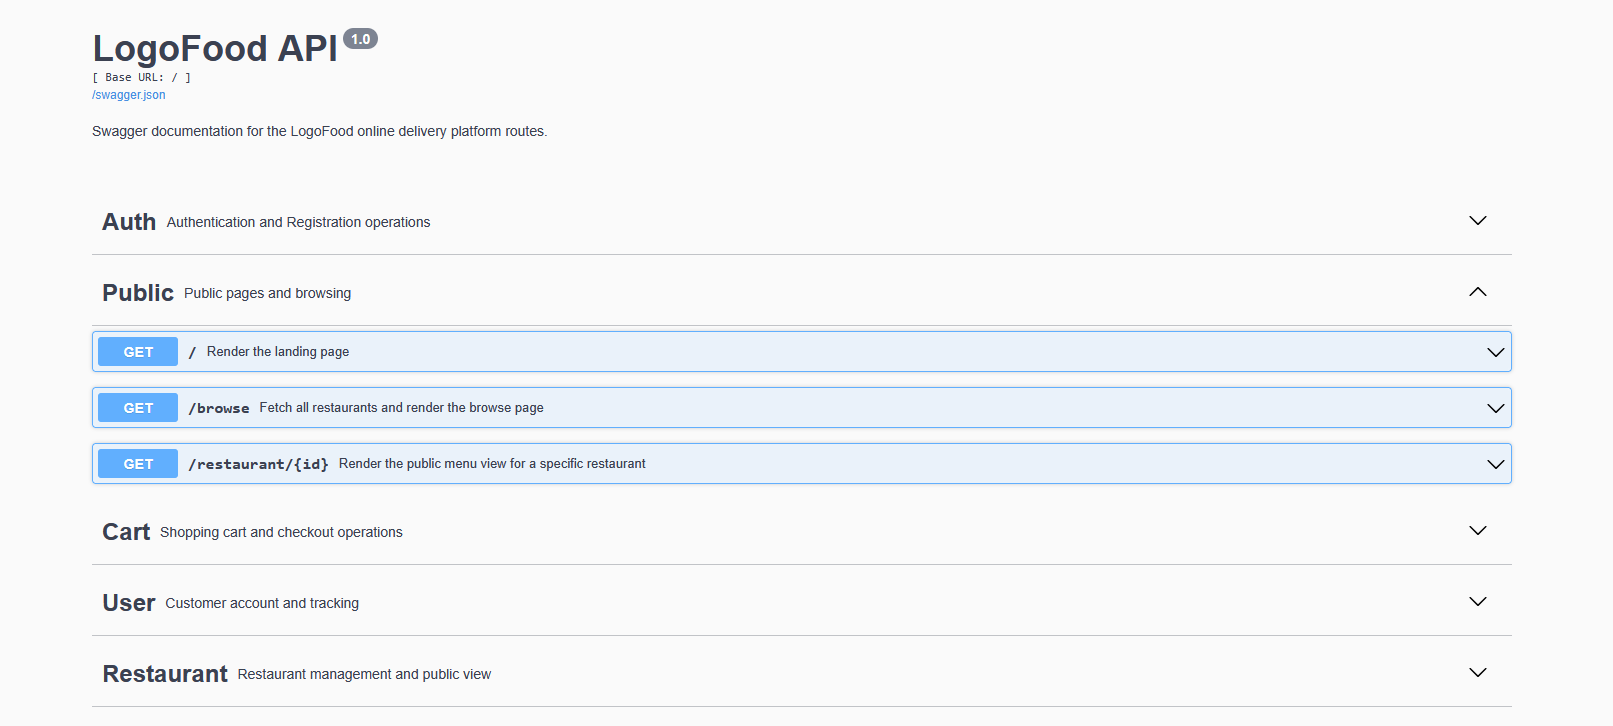
\includegraphics[width=0.9\linewidth]{images/swagger_routes.png}
		\caption{Απεικόνιση των routes της εφαρμογής στο Swagger UI.}
		\label{fig:swagger_routes}
	\end{figure}

	\begin{figure}[H]
		\centering
		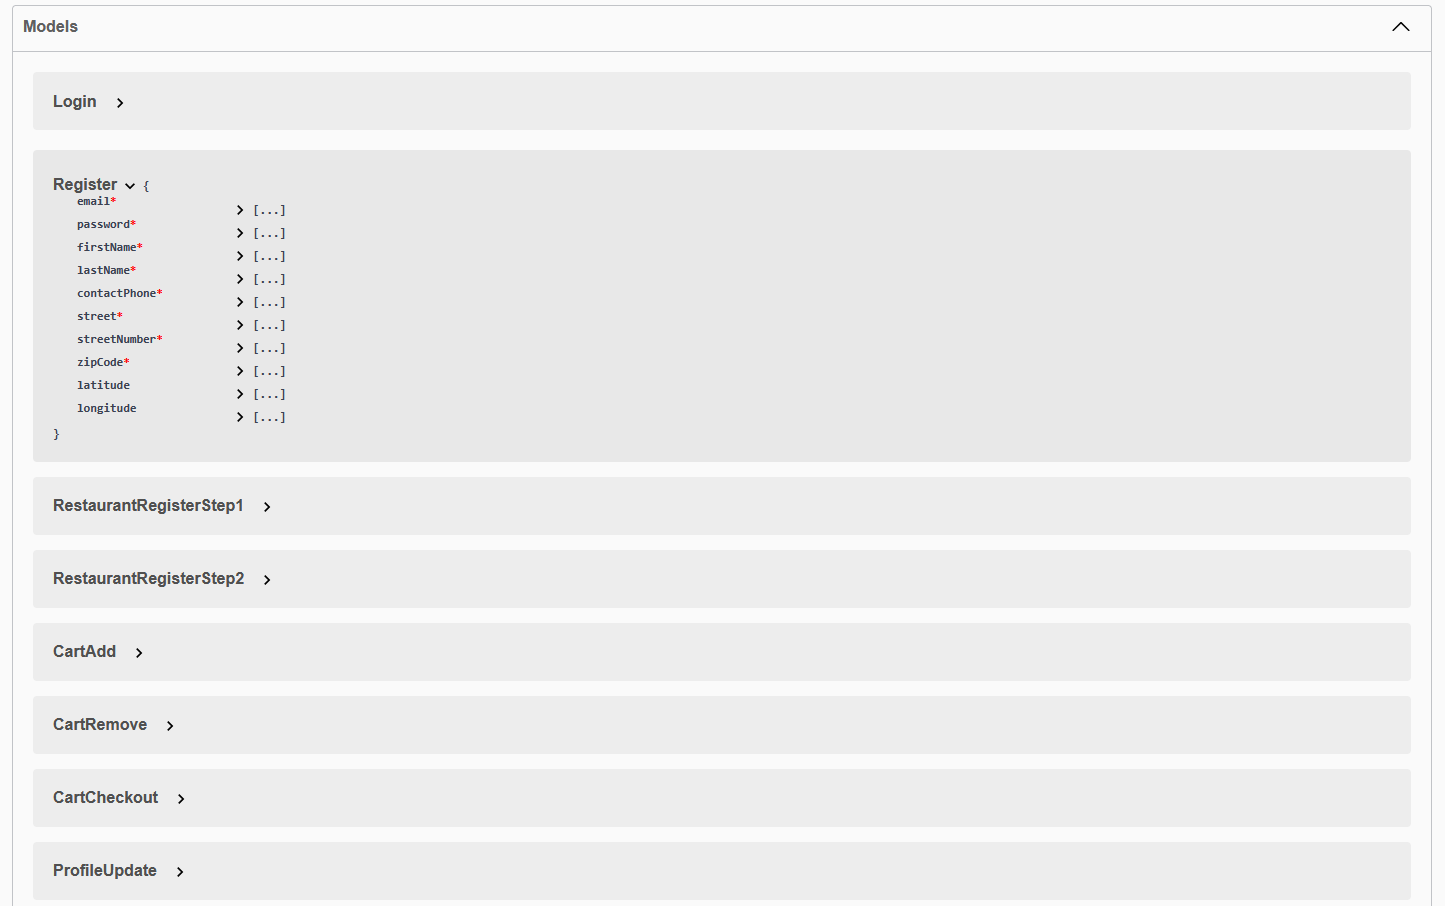
\includegraphics[width=0.9\linewidth]{images/swagger_models.png}
		\caption{Μοντέλα δεδομένων του API.}
		\label{fig:swagger_models}
	\end{figure}

	\section{Προβλήματα και Λύσεις που Εμφανίστηκαν}
	Κατά την ανάπτυξη του συστήματος παραγγελιών, αντιμετωπίστηκαν προκλήσεις που αφορούσαν τη διατήρηση του ιστορικού των παραγγελιών σε σχέση με τις διαγραφές δεδομένων από τους χρήστες.

	\subsection{Το Πρόβλημα της Διαγραφής Διευθύνσεων}
	Στο αρχικό σχήμα της βάσης δεδομένων, ο πίνακας \texttt{Order\_table} συνδεόταν με τον πίνακα \texttt{Address} μέσω ξένου κλειδιού. Η διαγραφή μιας διεύθυνσης από το προφίλ του χρήστη οδηγούσε στον μηδενισμό του πεδίου \texttt{delivery\_address\_id} (λόγω του κανόνα \texttt{ON DELETE SET NULL}).

	Αυτό προκάλεσε το φαινόμενο οι παραγγελίες να "εξαφανίζονται" από το ιστορικό του χρήστη, καθώς οι ερωτήσεις στη βάση χρησιμοποιούσαν \texttt{INNER JOIN}. Το πρόβλημα λύθηκε με τη μετάβαση σε \texttt{LEFT JOIN}, επιτρέποντας την εμφάνιση των παραγγελιών ακόμα και αν η διεύθυνση είχε διαγραφεί.

	\subsection{Διατήρηση Ιστορικού με Στιγμιότυπα (Snapshotting)}
	Παρά τη λύση του \texttt{LEFT JOIN}, αν η διεύθυνση είχε διαγραφεί, το σύστημα δεν μπορούσε να εμφανίσει πού είχε παραδοθεί η παραγγελία. Για την επίλυση αυτού, εφαρμόστηκε η τεχνική του \textbf{Snapshotting}.

	Προστέθηκε η στήλη \texttt{delivery\_address\_text} στον πίνακα \texttt{Order\_table}. Κατά τη δημιουργία της παραγγελίας, η πλήρης διεύθυνση αποθηκεύεται ως κείμενο απευθείας στην παραγγελία. Έτσι, ακόμα και αν ο χρήστης διαγράψει ή τροποποιήσει τη διεύθυνσή του στο μέλλον, το ιστορικό της παραγγελίας παραμένει αναλλοίωτο και ακριβές.

	\section{Συμπεράσματα}
	Η ενασχόληση με το project LogoFood προσέφερε πολύτιμη εμπειρία σε όλο το φάσμα της ανάπτυξης διαδικτυακών εφαρμογών, από το σχεδιασμό της εμπειρίας χρήστη (UX) μέχρι την επίλυση σύνθετων προβλημάτων στο backend και τη διαχείριση cloud υποδομών.
	
	\section{Οδηγίες Εγκατάστασης και Εκκίνησης}
	\begin{enumerate}
		\item \textbf{Εφαρμογή (Node.js):}
		\begin{itemize}
			\item Μεταβείτε στον φάκελο \texttt{logofood-app}.
			\item Εκτελέστε \texttt{npm install} για την εγκατάσταση των εξαρτήσεων.
			\item Δημιουργήστε αρχείο \texttt{.env} με τις απαραίτητες ρυθμίσεις για τη βάση δεδομένων.
			\item Εκτελέστε \texttt{npm start} για την εκκίνηση του server.
		\end{itemize}
		\item \textbf{Τεκμηρίωση API (Python):}
		\begin{itemize}
			\item Μεταβείτε στον φάκελο \texttt{python}.
			\item Εκτελέστε \texttt{pip install -r requirements.txt} (αν απαιτείται).
			\item Εκτελέστε \texttt{python swagger\_api.py} για την εκκίνηση του Swagger UI.
		\end{itemize}
	\end{enumerate}
	
	\section{Σύνδεσμοι Έργου}
	\begin{itemize}
		\item \textbf{GitHub:} \url{https://github.com/jimfil/onlineFoodDeliveryApplication}
		\item \textbf{Ιστοσελίδα στο Render:} \url{https://onlinefooddeliveryapplication.onrender.com}
	\end{itemize}
	
	\appendix

	\section{Στιγμιότυπα Εφαρμογής}

	\begin{figure}[H]
		\centering
		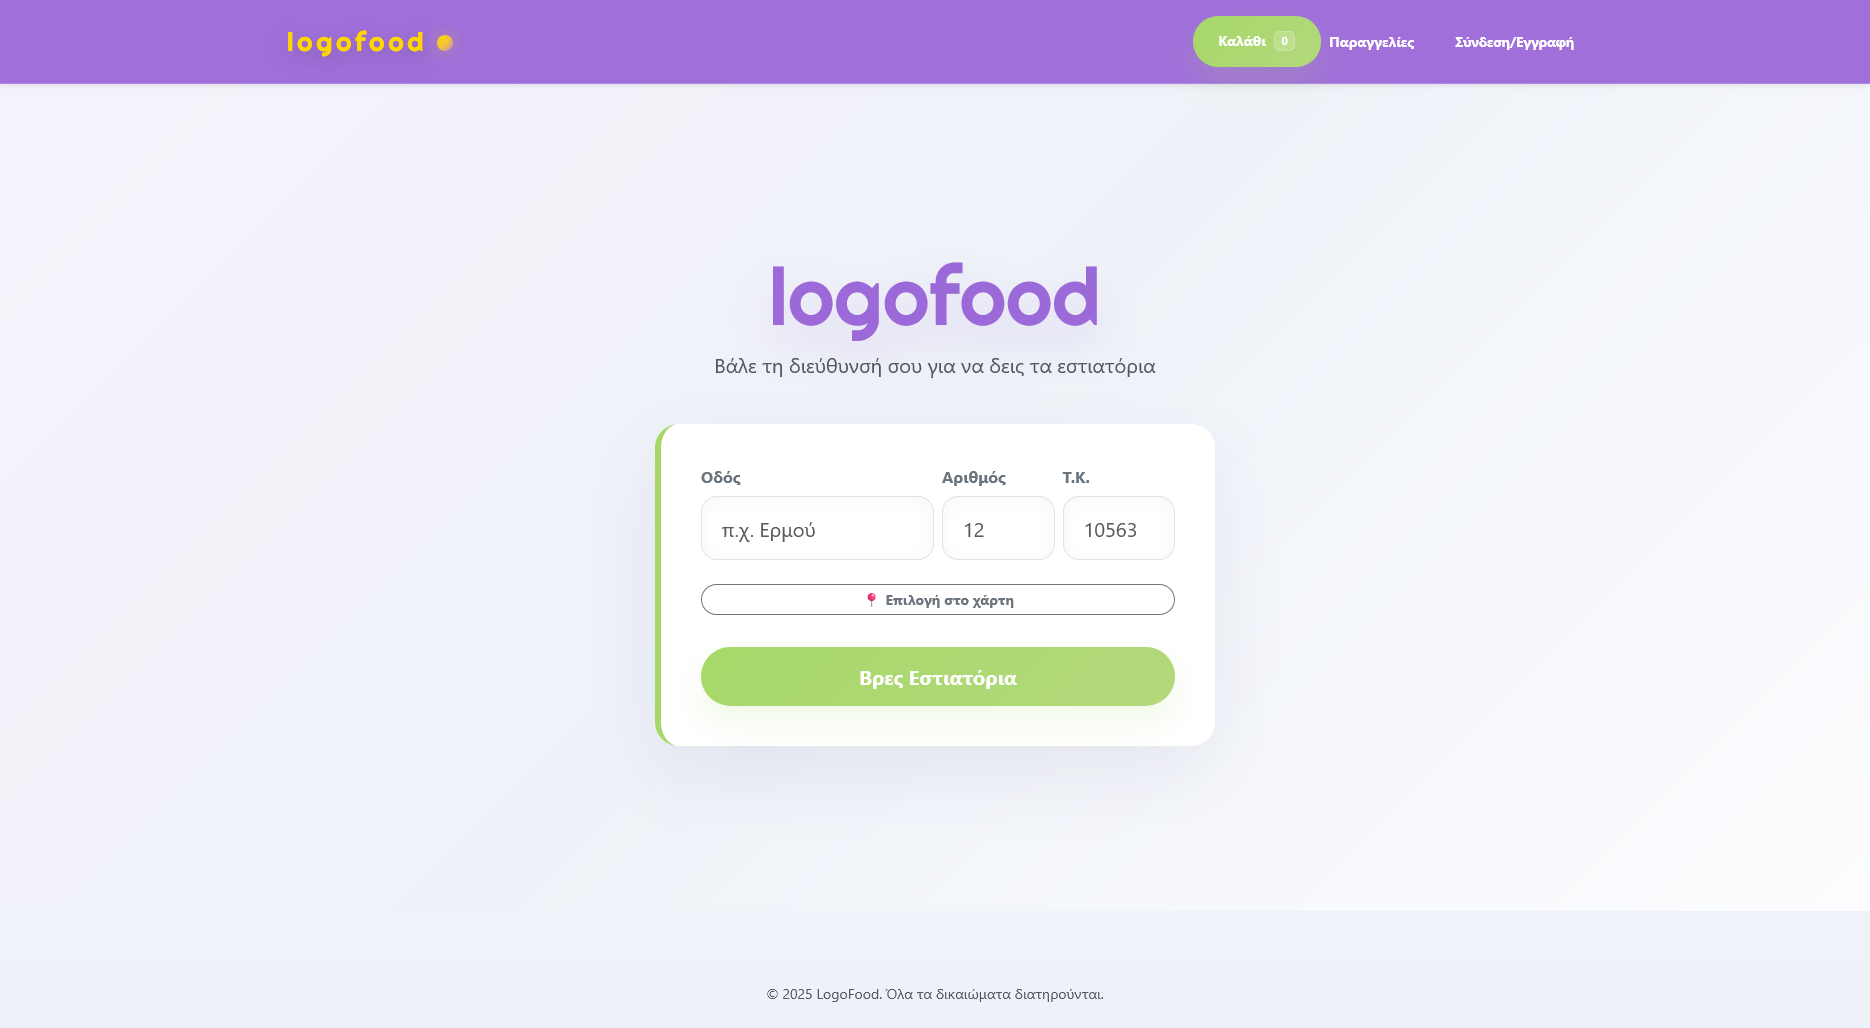
\includegraphics[width=0.9\linewidth]{images/indexPage.png}
		\caption{Αρχική σελίδα (Landing Page) της εφαρμογής.}
	\end{figure}

	\begin{figure}[H]
		\centering
		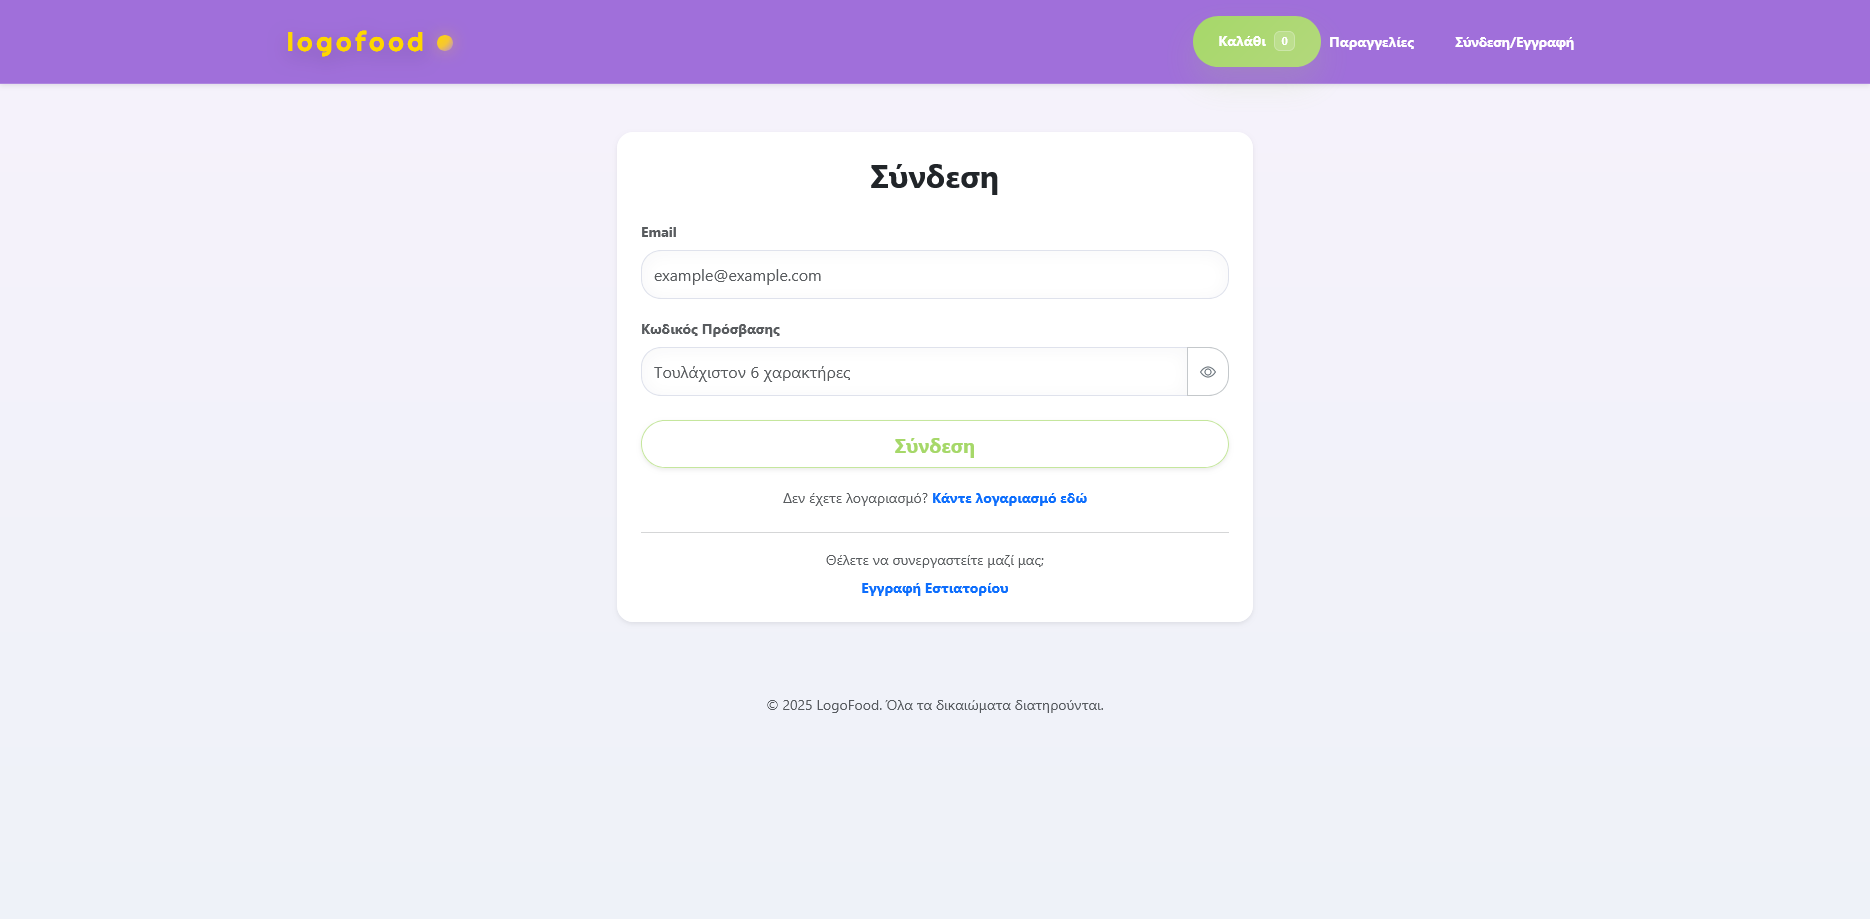
\includegraphics[width=0.9\linewidth]{images/loginPage.png}
		\caption{Σελίδα σύνδεσης χρηστών.}
	\end{figure}

	\begin{figure}[H]
		\centering
		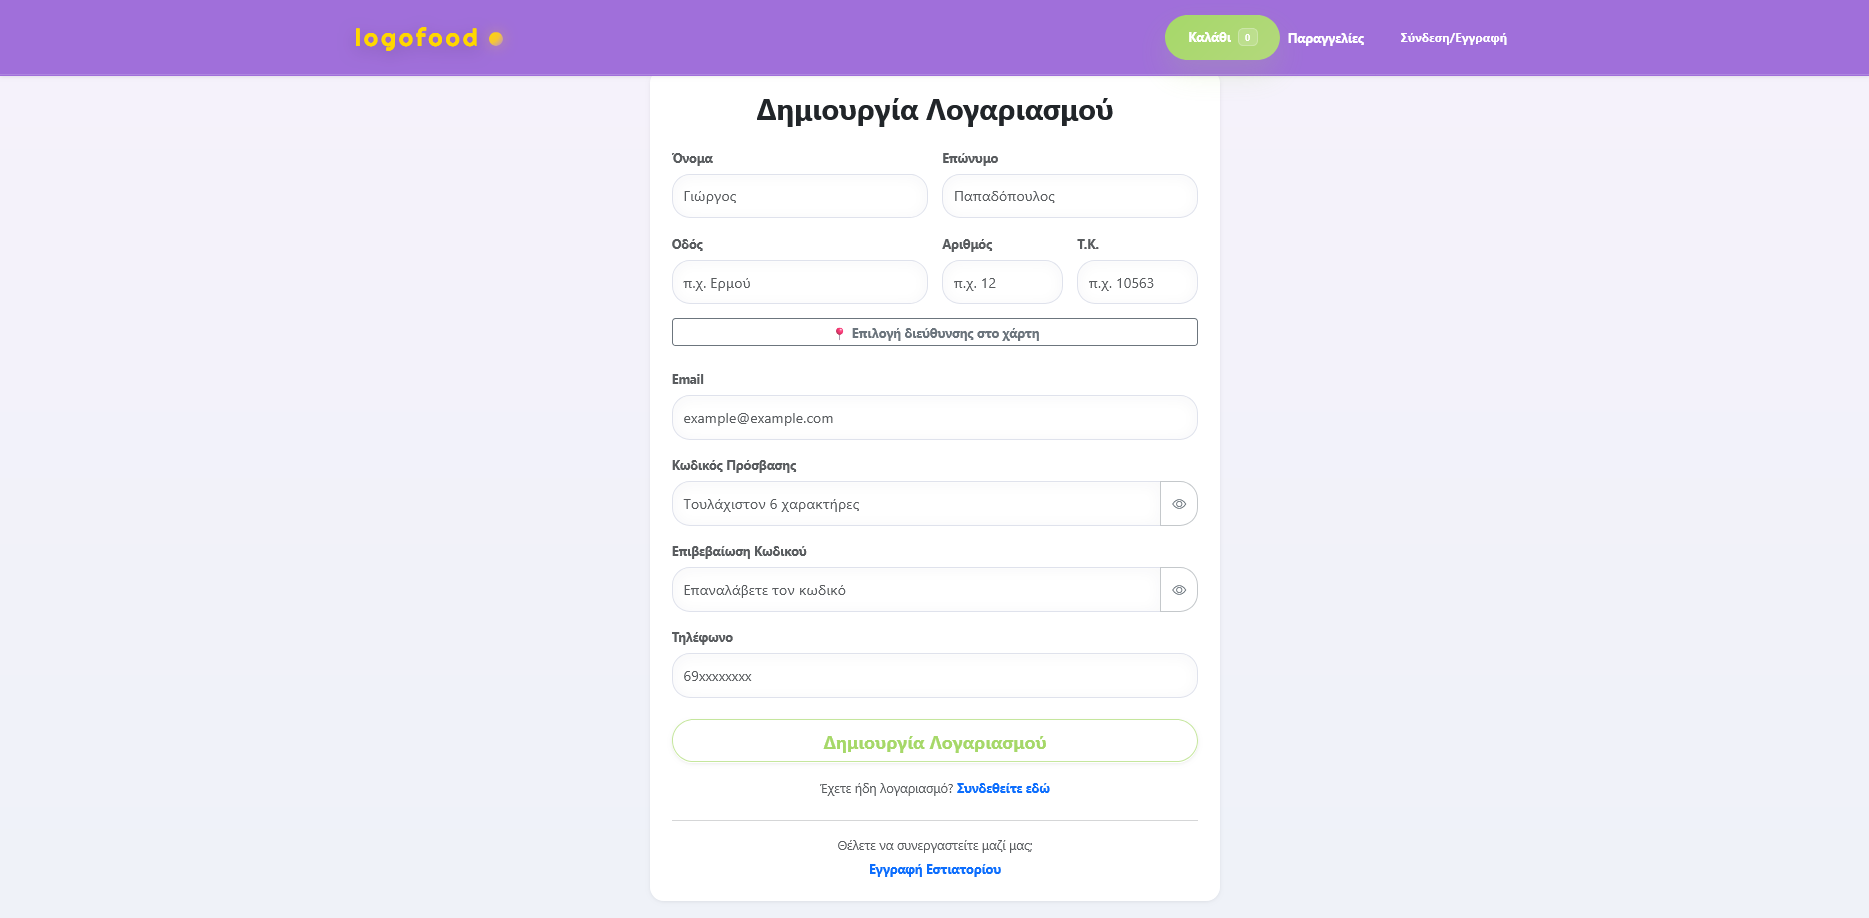
\includegraphics[width=0.9\linewidth]{images/registerPage.png}
		\caption{Σελίδα εγγραφής νέου πελάτη.}
	\end{figure}

	\begin{figure}[H]
		\centering
		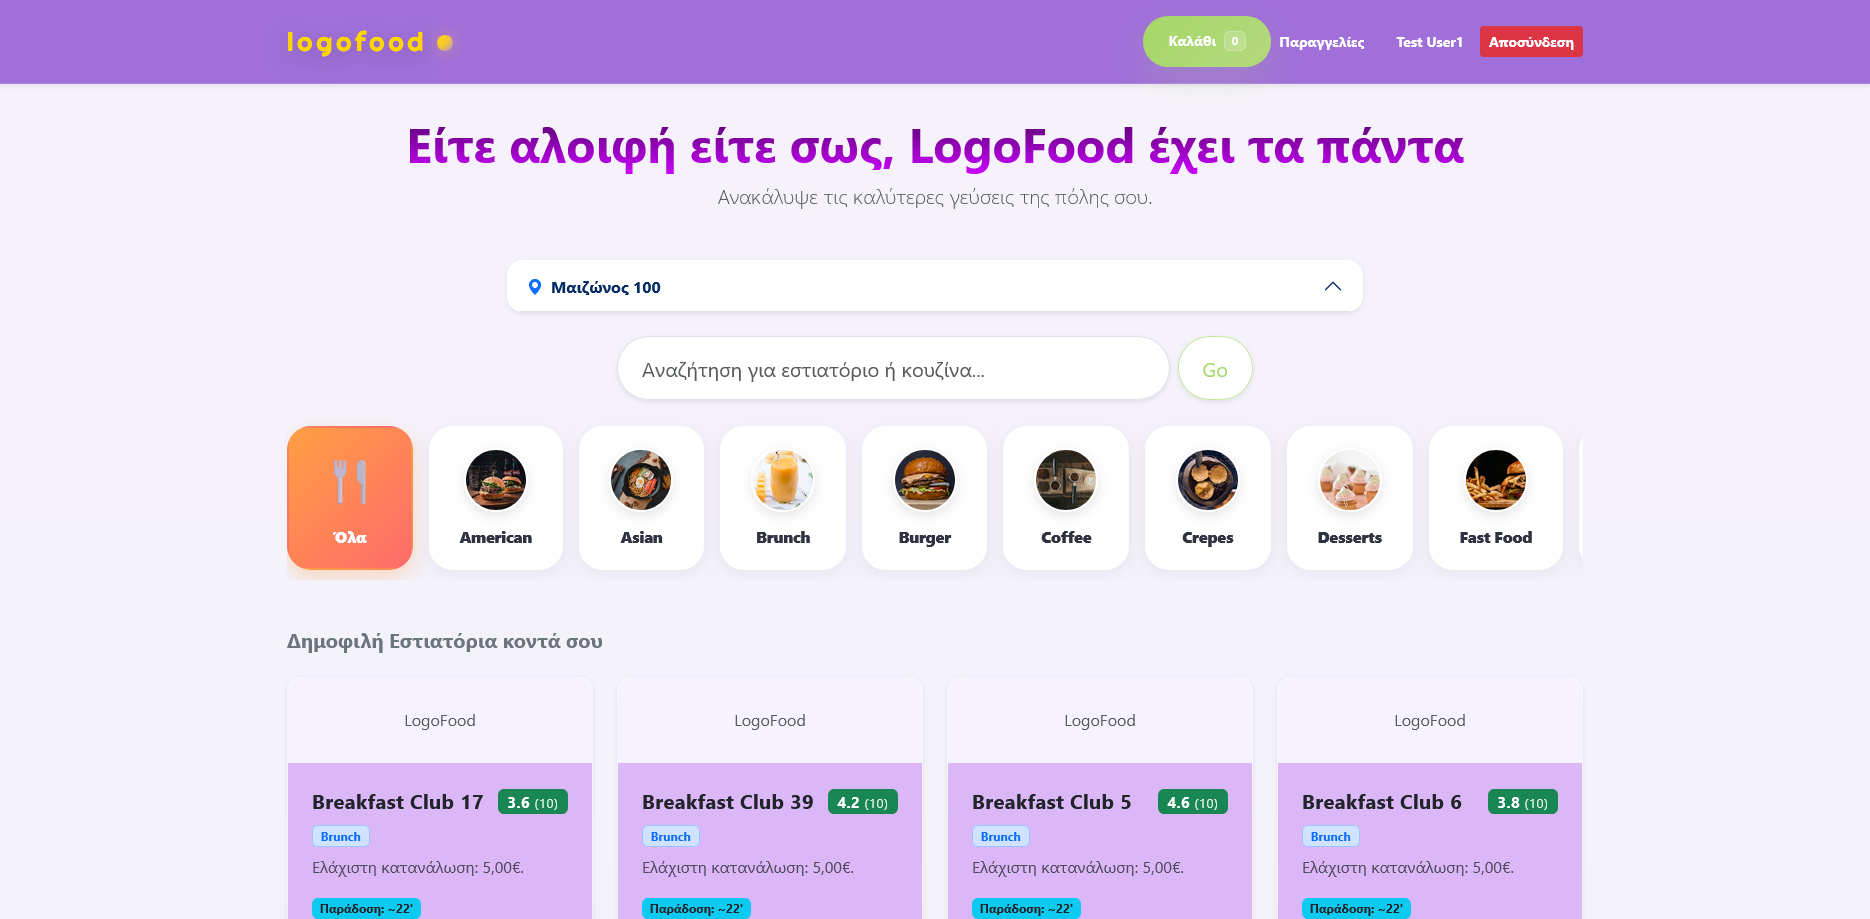
\includegraphics[width=0.9\linewidth]{images/browsePage.png}
		\caption{Σελίδα αναζήτησης εστιατορίων με φίλτρα κατηγοριών.}
	\end{figure}

	\begin{figure}[H]
		\centering
		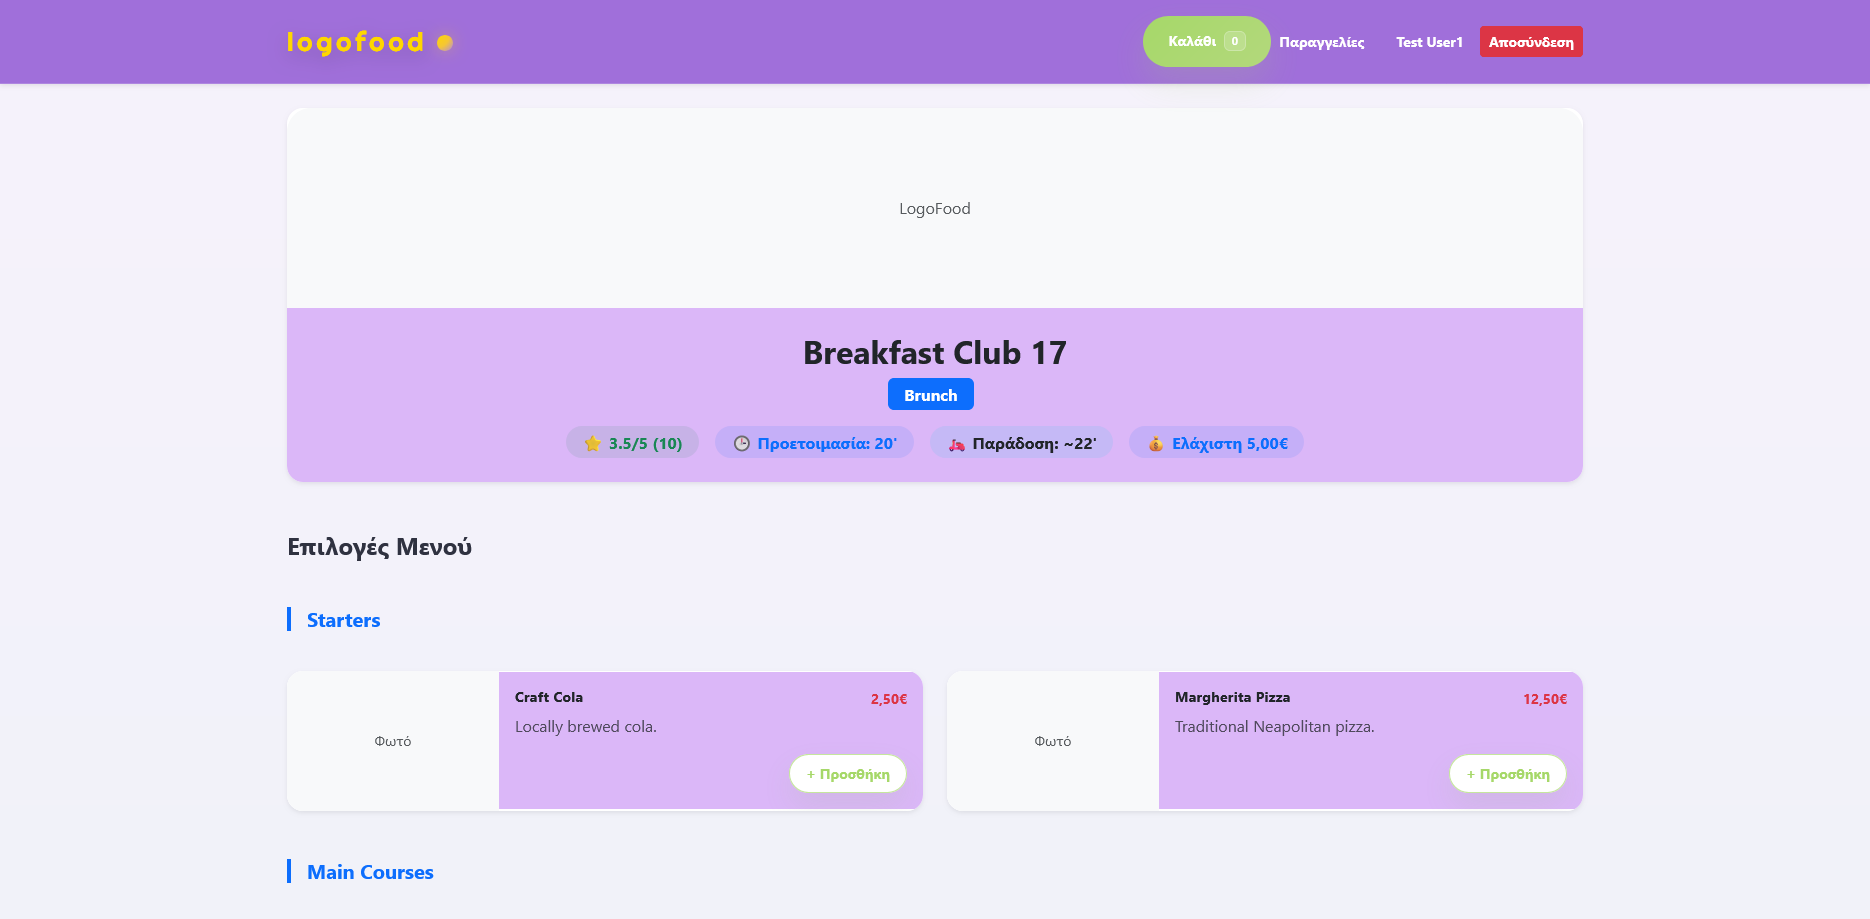
\includegraphics[width=0.9\linewidth]{images/restaurantPage.png}
		\caption{Σελίδα εστιατορίου με μενού προϊόντων.}
	\end{figure}

	\begin{figure}[H]
		\centering
		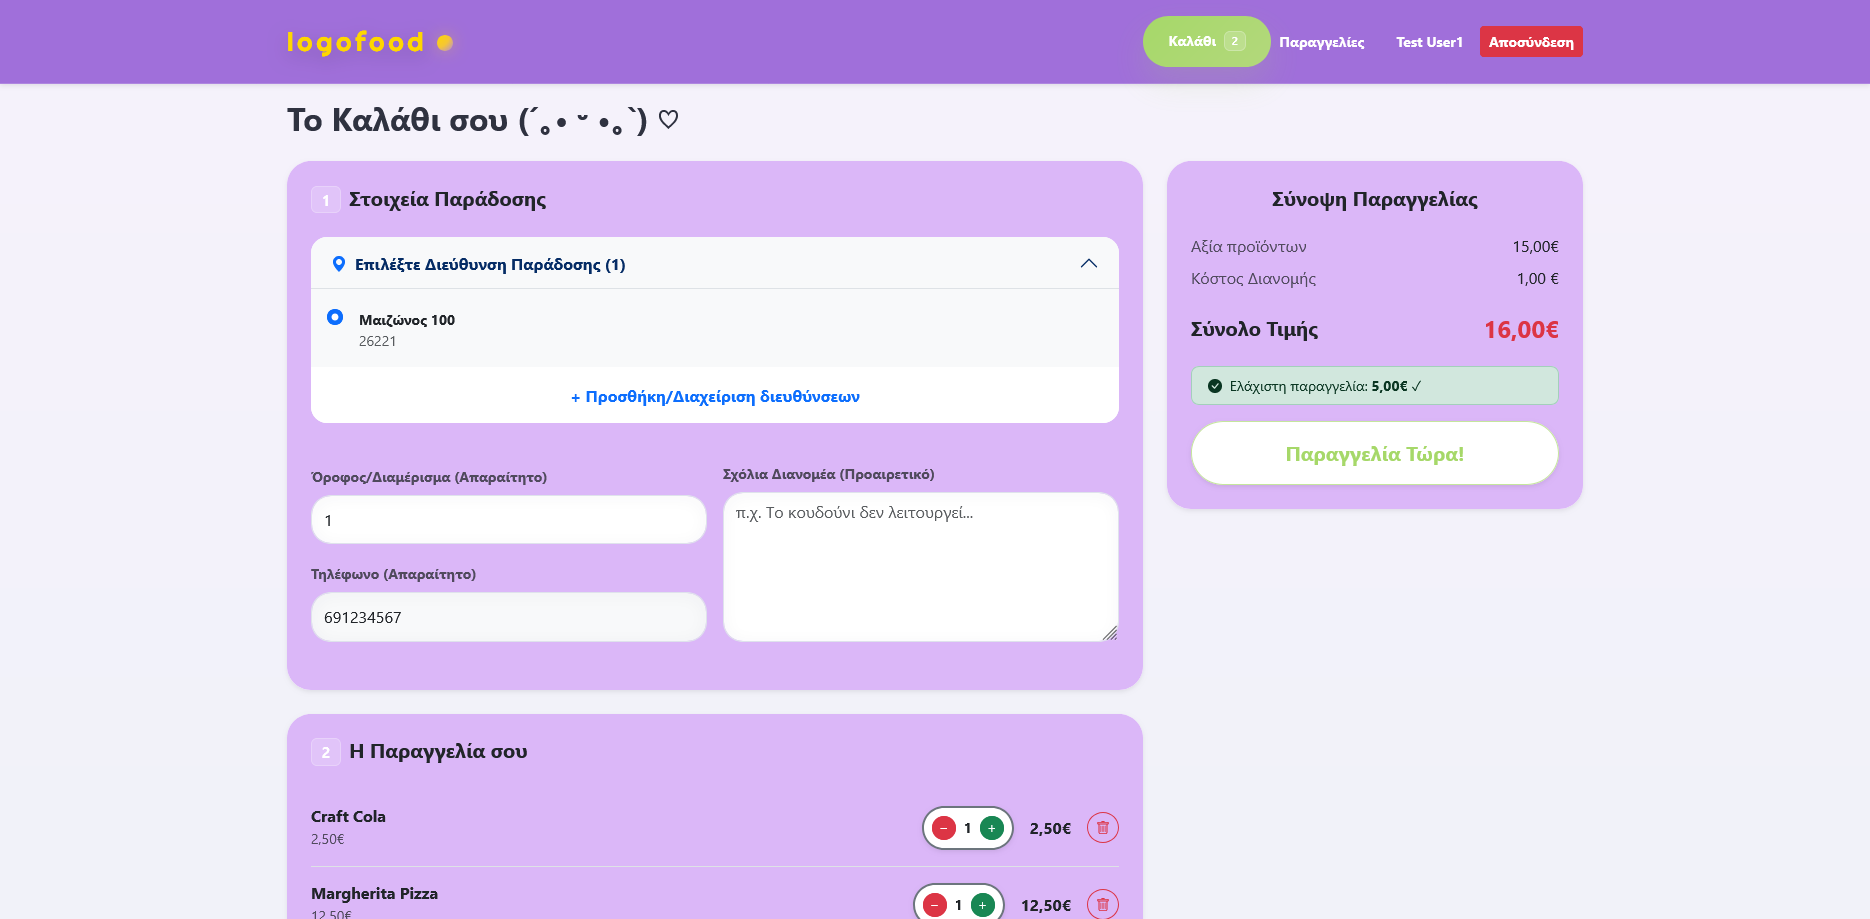
\includegraphics[width=0.9\linewidth]{images/cartPage.png}
		\caption{Σελίδα καλαθιού αγορών και ολοκλήρωσης παραγγελίας.}
	\end{figure}

	\begin{figure}[H]
		\centering
		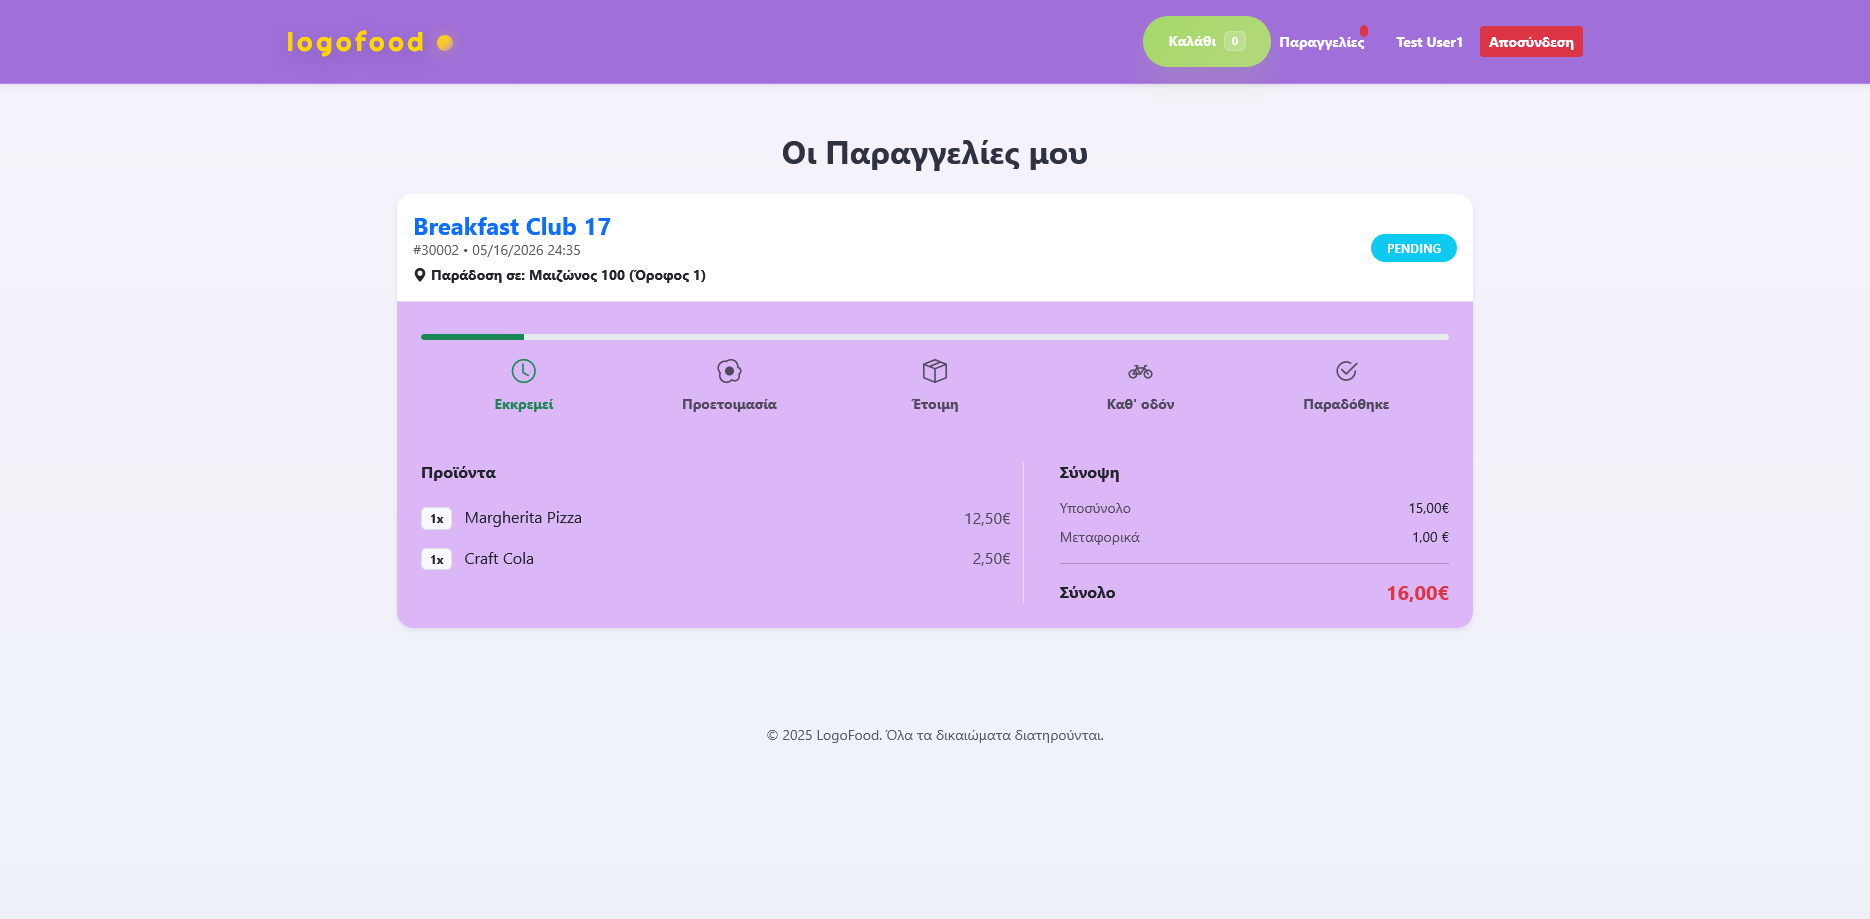
\includegraphics[width=0.9\linewidth]{images/trackingOrderPage.png}
		\caption{Σελίδα παρακολούθησης παραγγελίας σε εξέλιξη.}
	\end{figure}

	\begin{figure}[H]
		\centering
		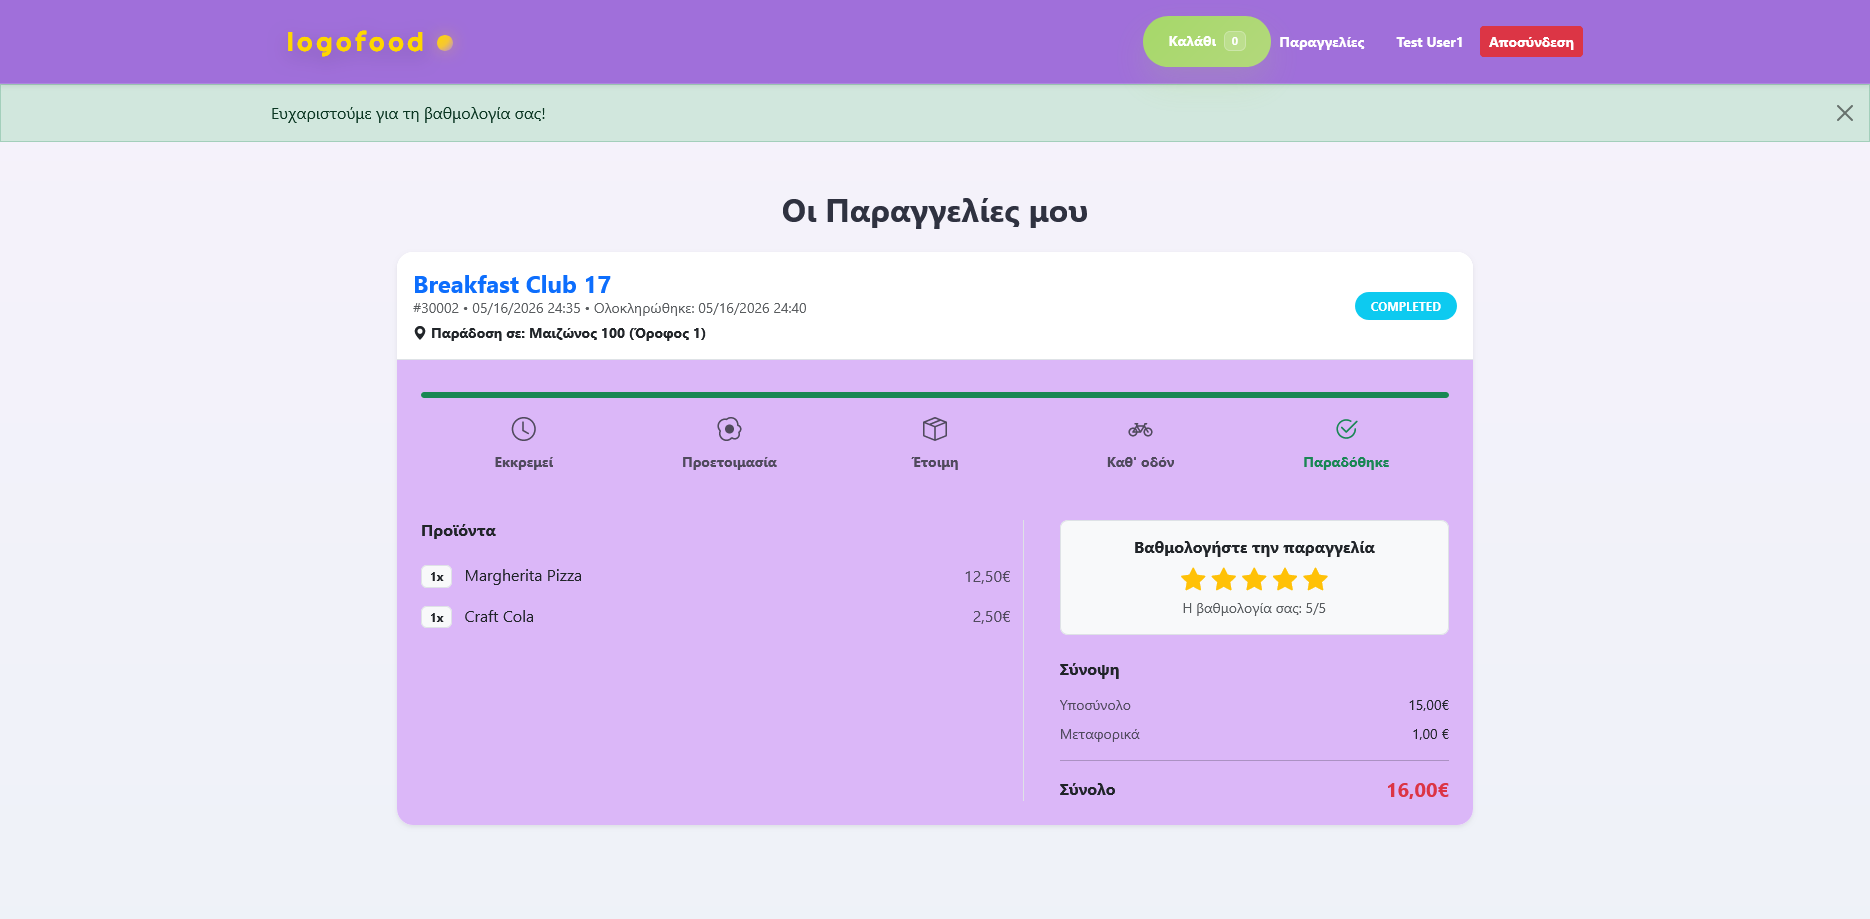
\includegraphics[width=0.9\linewidth]{images/TrackordersPostcompetionAndSubmitionPage.png}
		\caption{Σελίδα παρακολούθησης παραγγελίας μετά την ολοκλήρωση και υποβολή αξιολόγησης.}
	\end{figure}

	\begin{figure}[H]
		\centering
		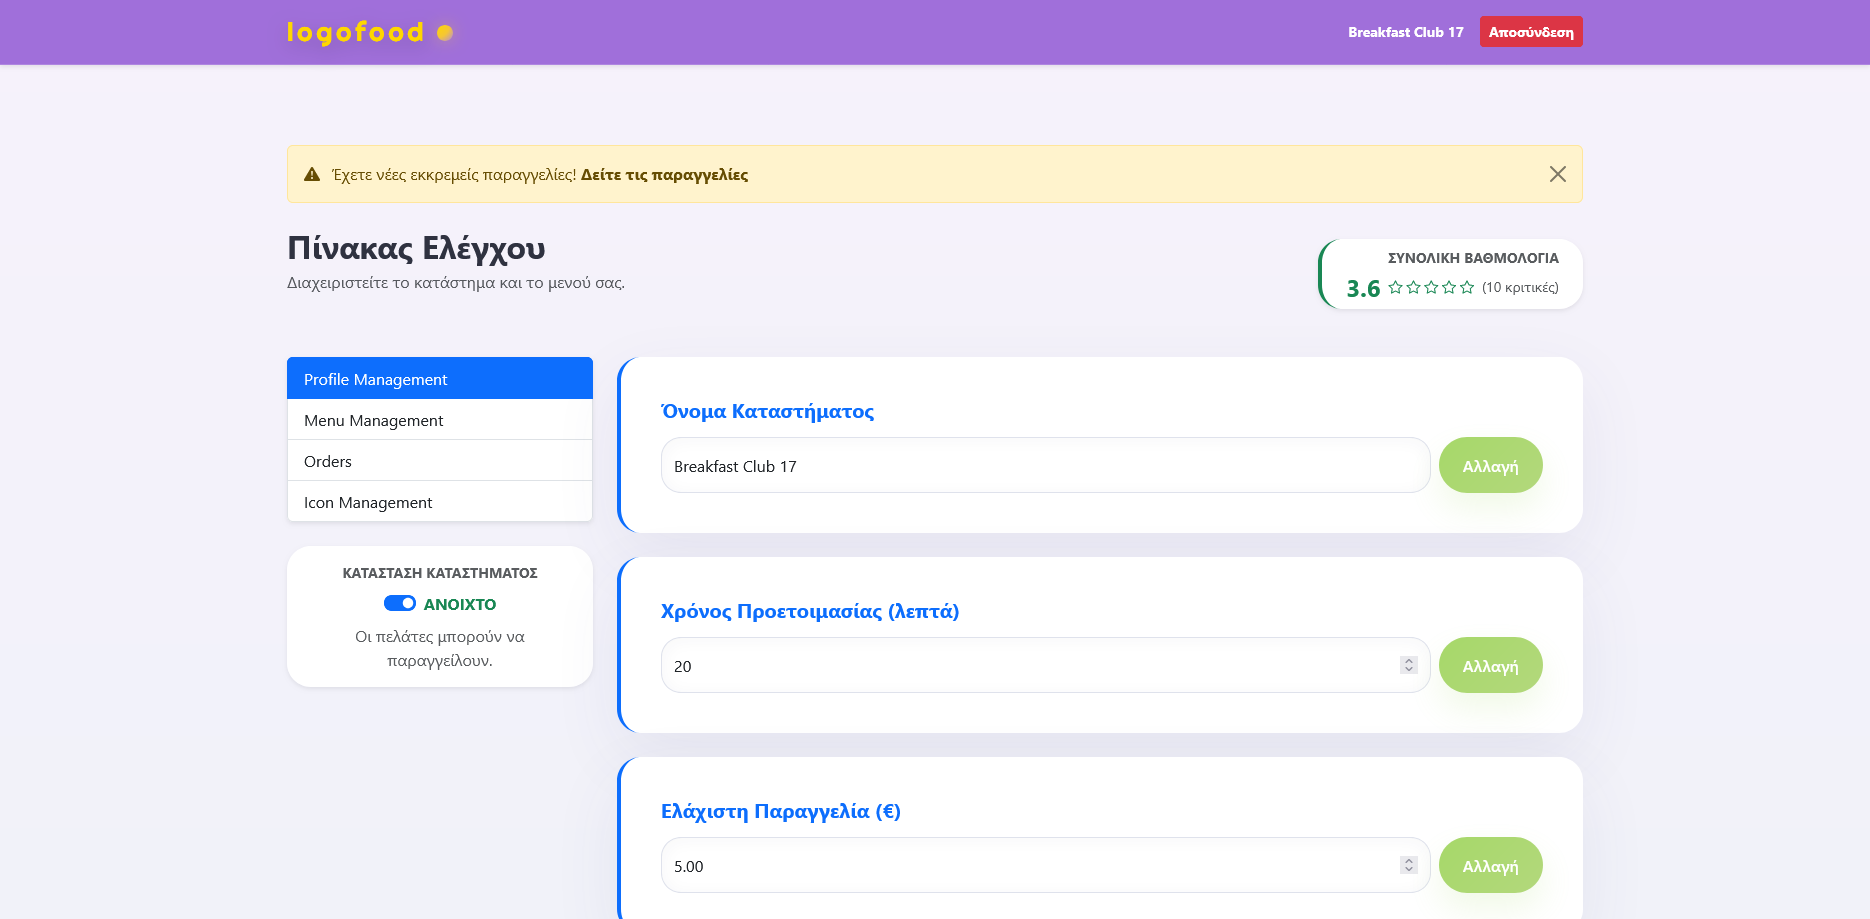
\includegraphics[width=0.9\linewidth]{images/restarauntManagePage.png}
		\caption{Dashboard διαχείρισης εστιατορίου — Προφίλ.}
	\end{figure}

	\begin{figure}[H]
		\centering
		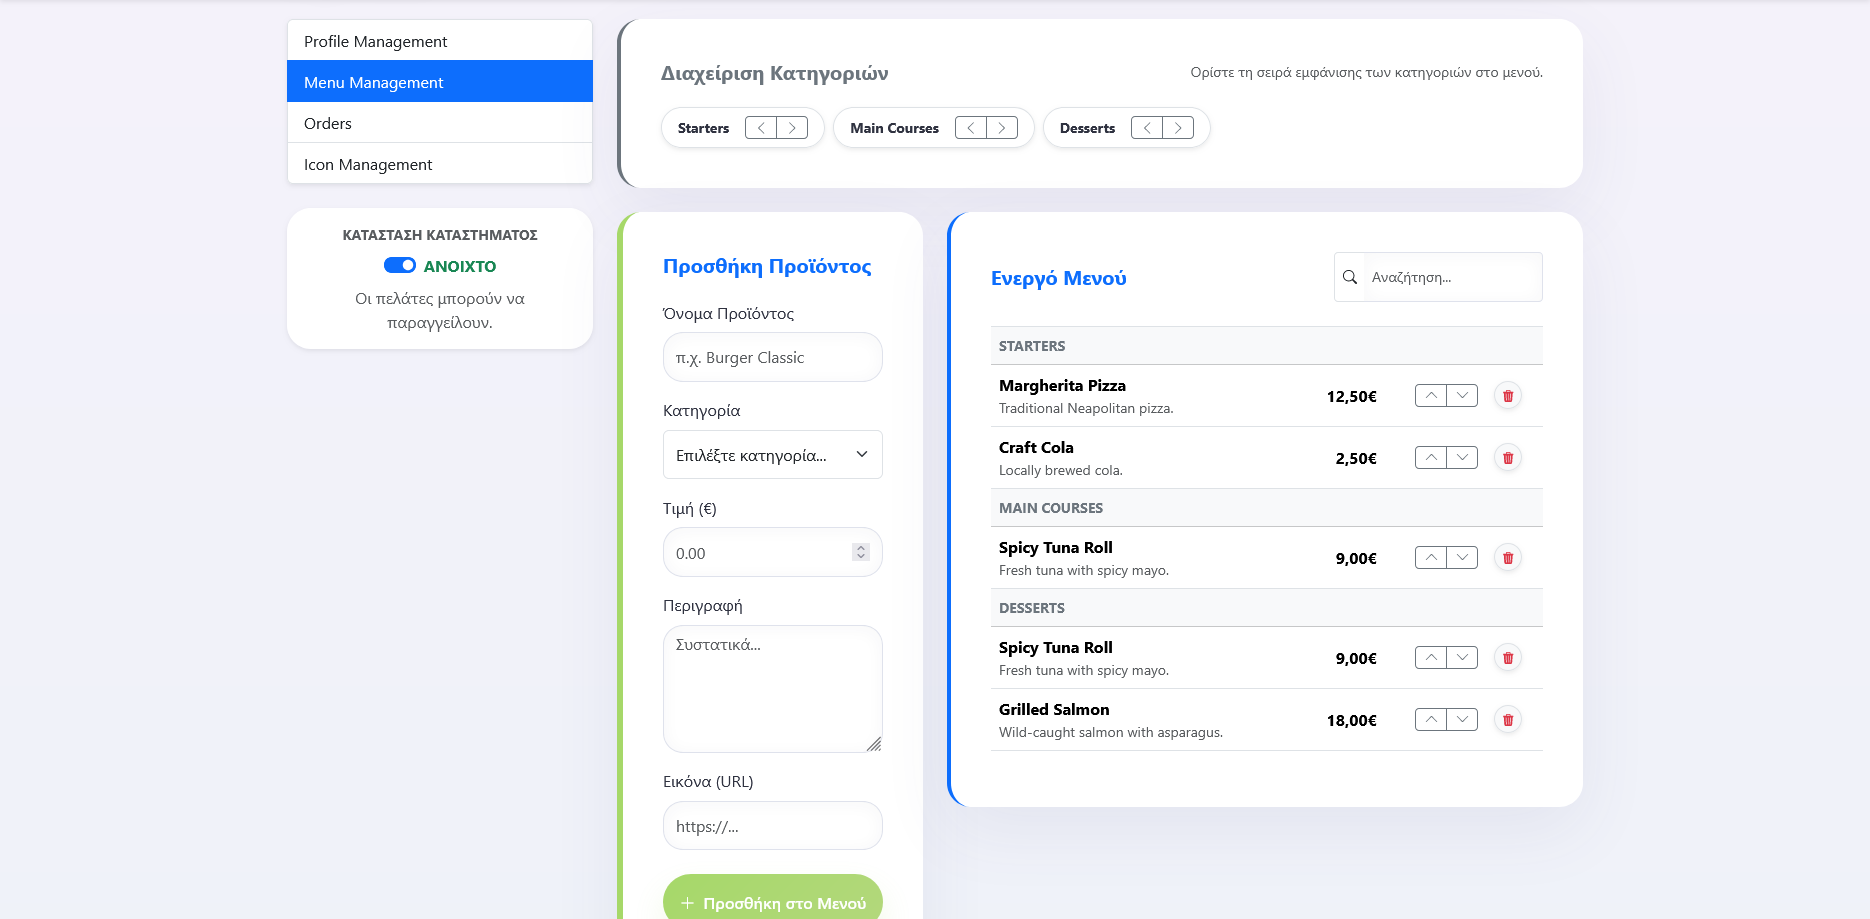
\includegraphics[width=0.9\linewidth]{images/menuManagementPage.png}
		\caption{Dashboard διαχείρισης εστιατορίου — Διαχείριση μενού.}
	\end{figure}

	\begin{figure}[H]
		\centering
		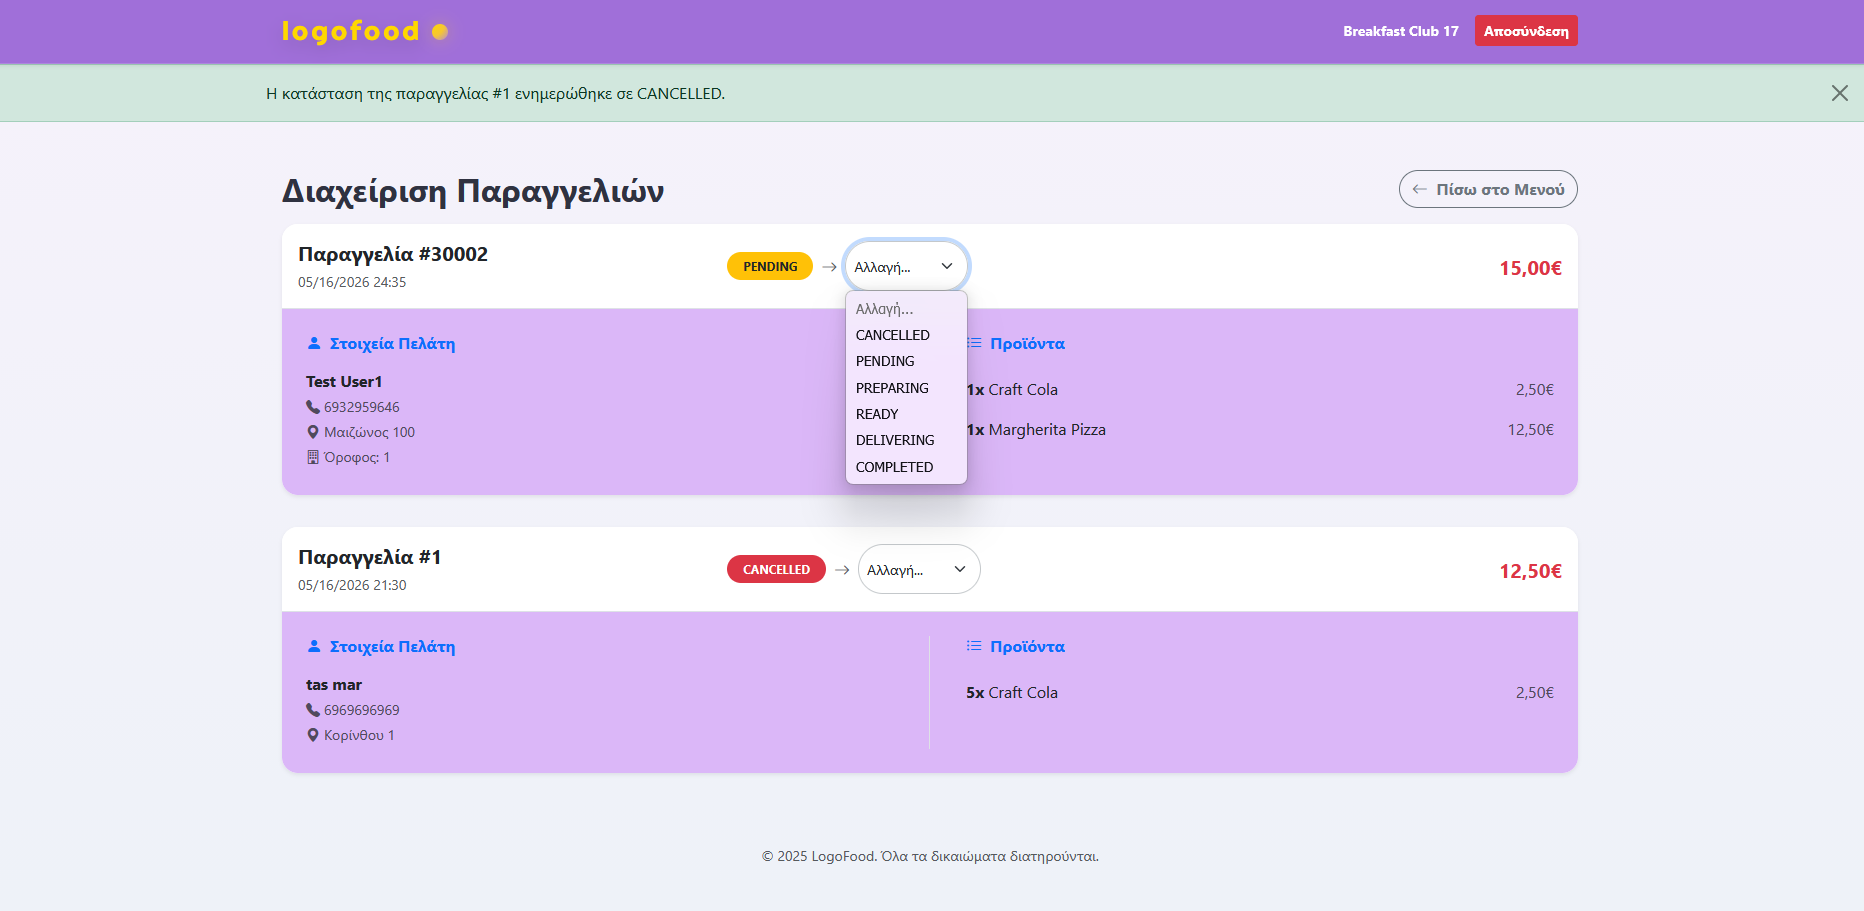
\includegraphics[width=0.9\linewidth]{images/restaurantOrdersPage.png}
		\caption{Σελίδα διαχείρισης παραγγελιών εστιατορίου.}
	\end{figure}

	\begin{figure}[H]
		\centering
		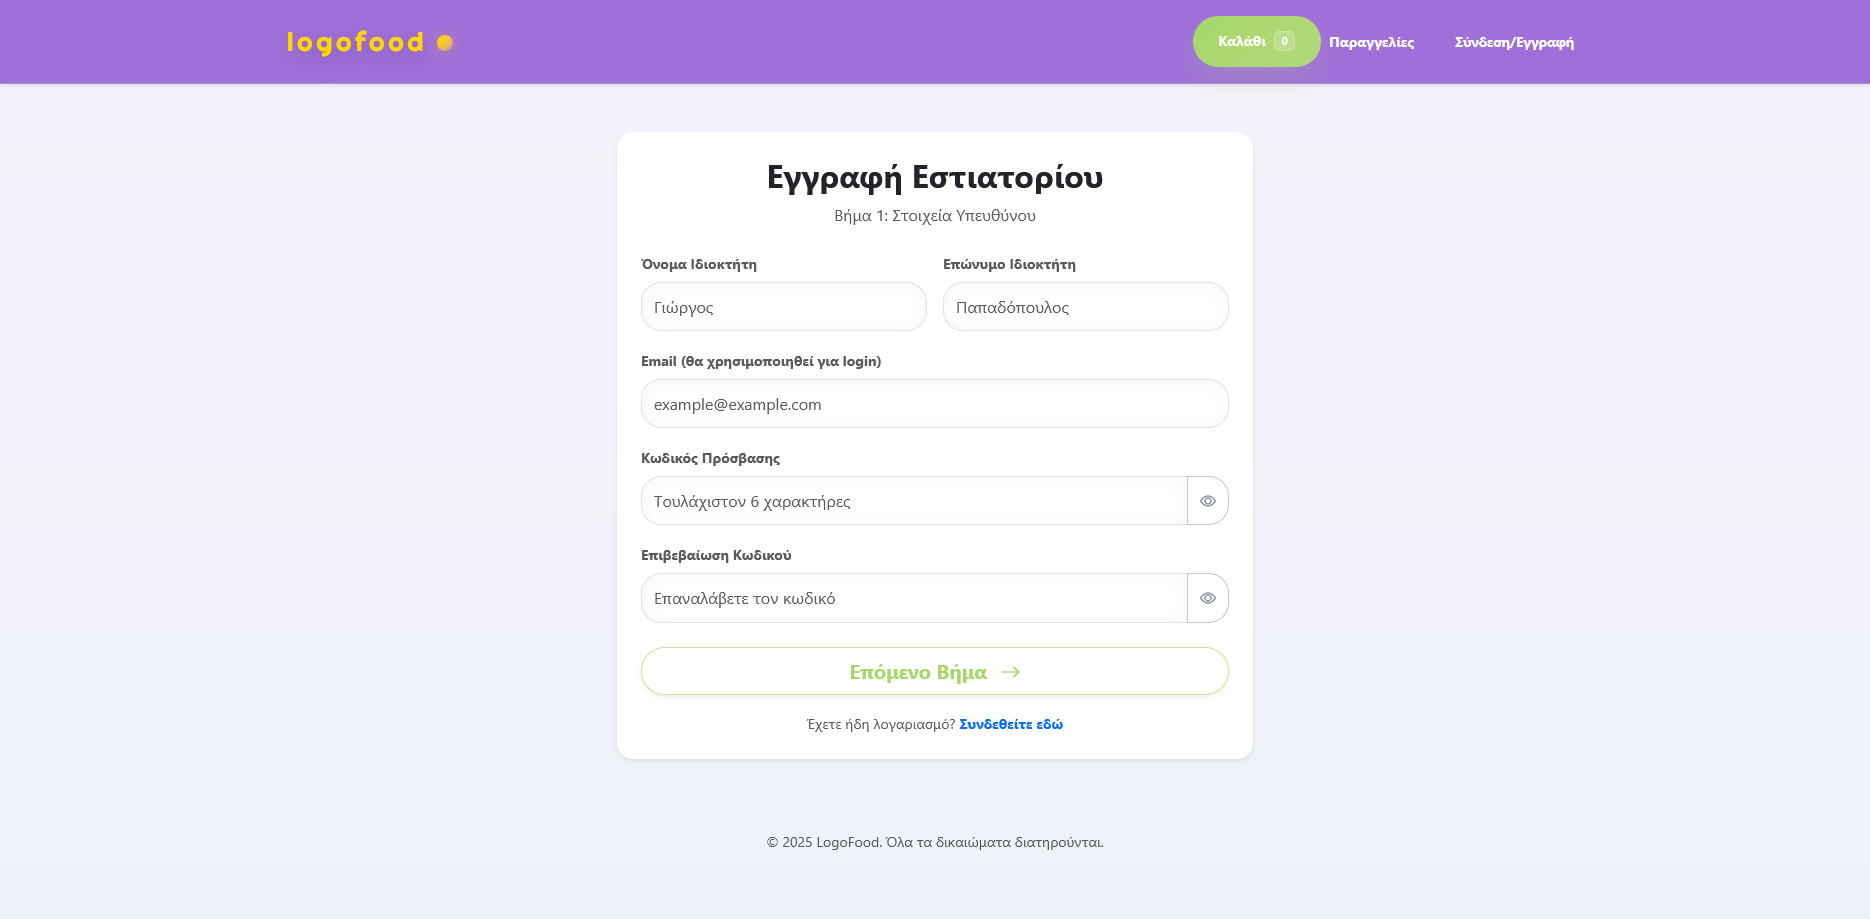
\includegraphics[width=0.9\linewidth]{images/registerRestaurantpart1.png}
		\caption{Εγγραφή εστιατορίου — Βήμα 1: Στοιχεία ιδιοκτήτη.}
	\end{figure}

	\begin{figure}[H]
		\centering
		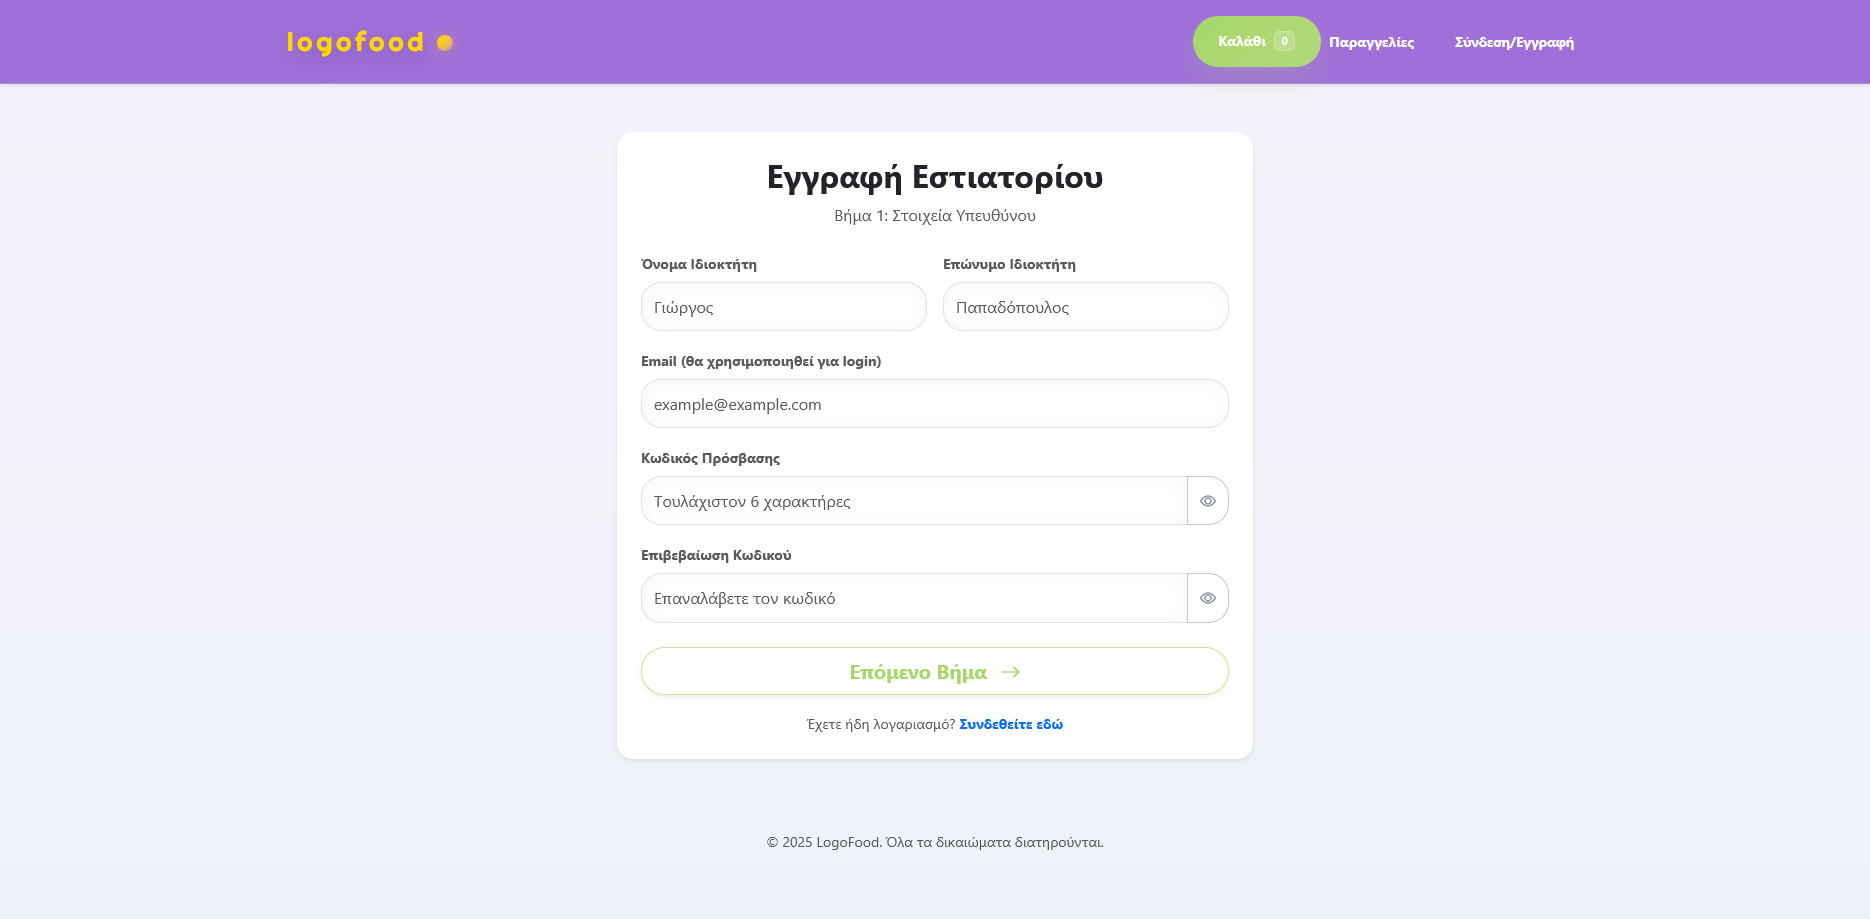
\includegraphics[width=0.9\linewidth]{images/registerRestaurantpart2.png}
		\caption{Εγγραφή εστιατορίου — Βήμα 2: Στοιχεία επιχείρησης.}
	\end{figure}

	\begin{figure}[H]
		\centering
		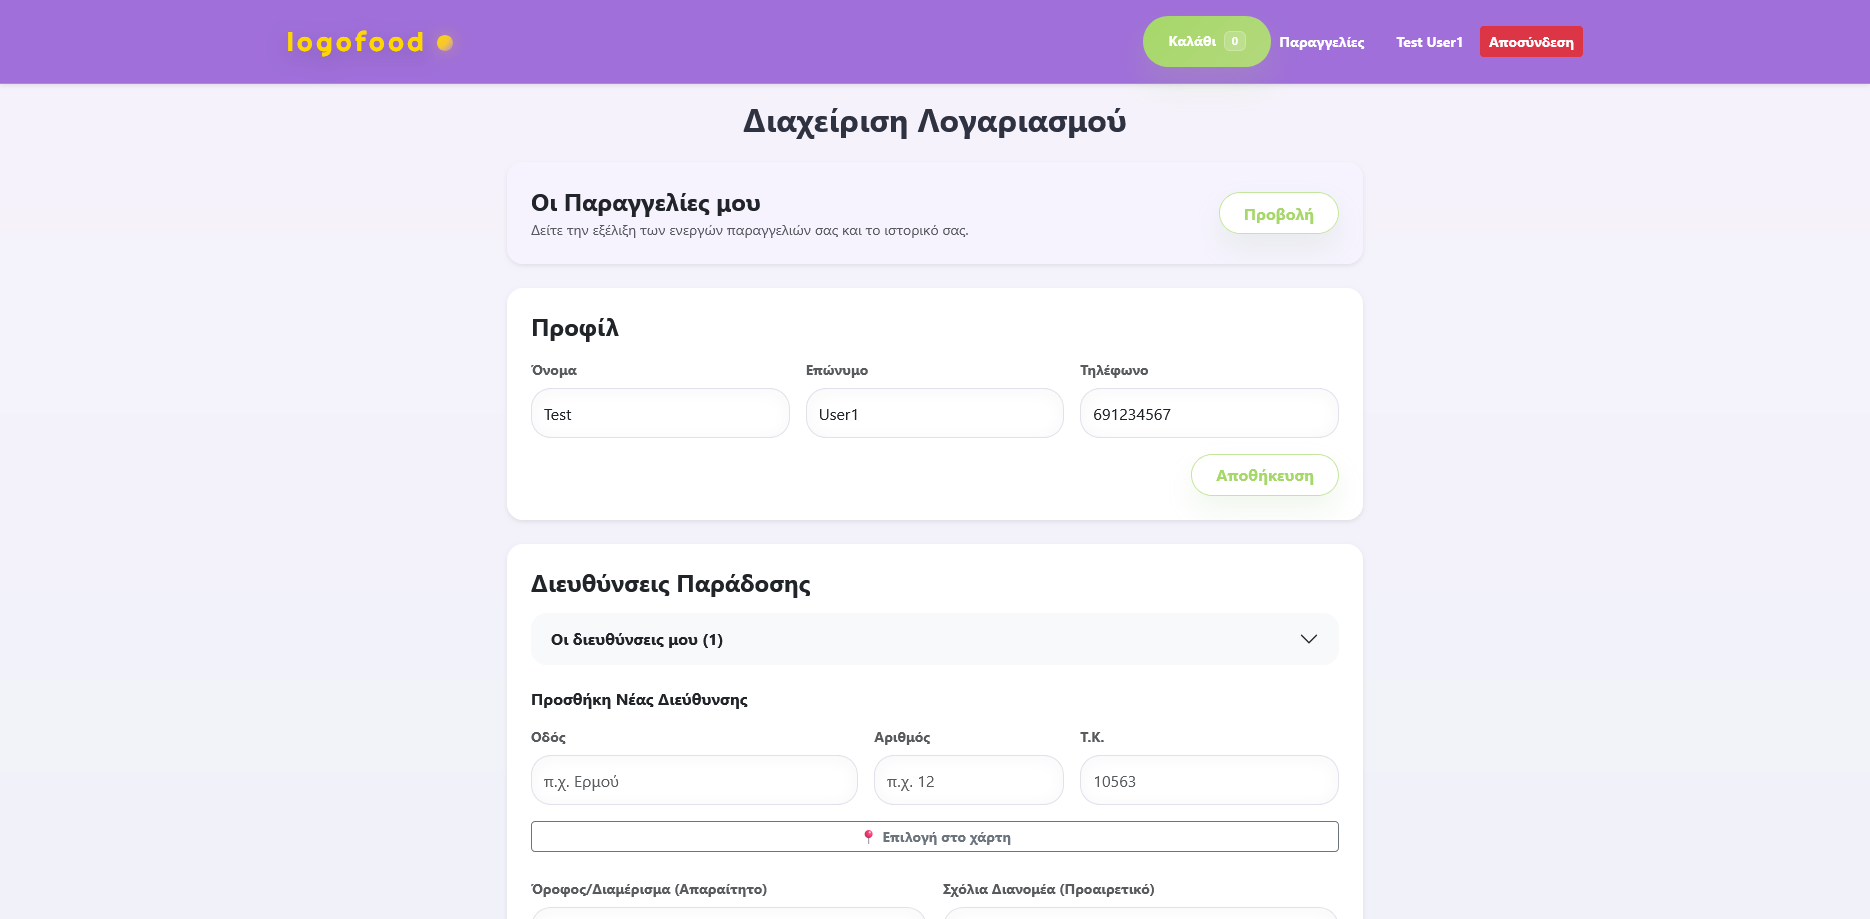
\includegraphics[width=0.9\linewidth]{images/usermanagementpage.png}
		\caption{Σελίδα διαχείρισης λογαριασμού χρήστη.}
	\end{figure}

	\begin{figure}[H]
		\centering
		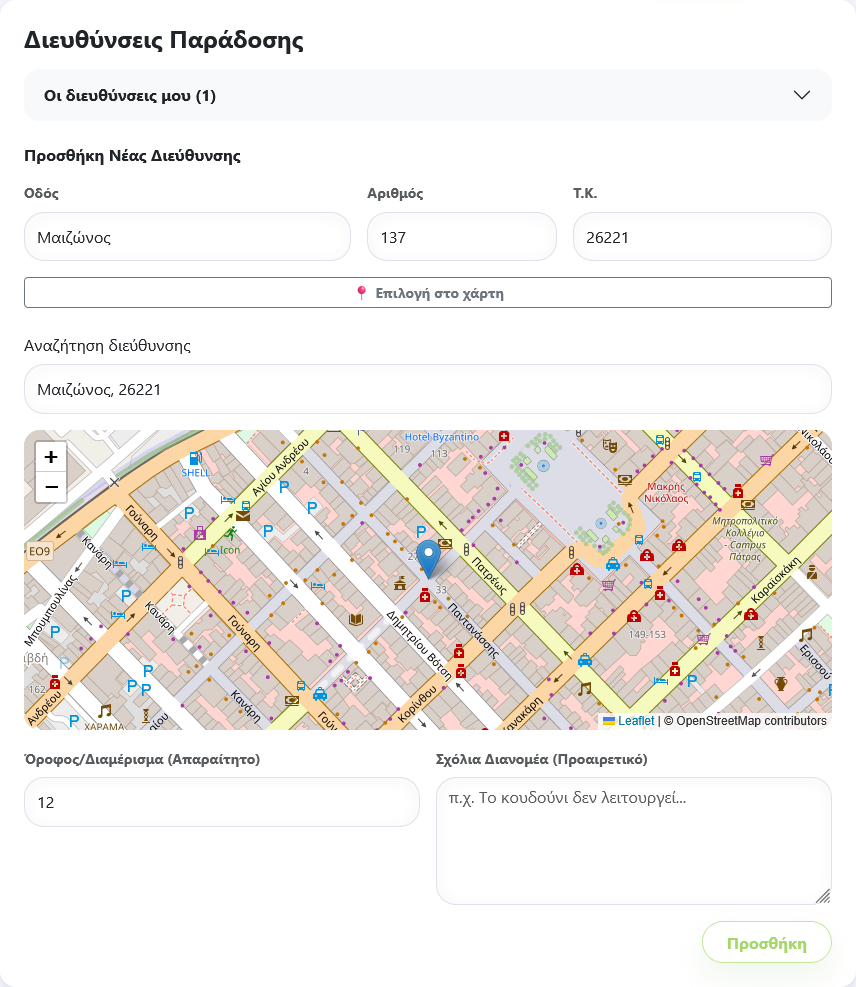
\includegraphics[width=0.9\linewidth]{images/addressEditManagement.png}
		\caption{Διαχείριση και επεξεργασία αποθηκευμένων διευθύνσεων.}
	\end{figure}

\end{document}